\section[SSU-ALIGN's SSU rRNA sequence and structure models]{SSU-ALIGN's SSU rRNA sequence and structure
  models\footnote{This is a slightly modified version 
  of a section from chapter 9 of my Ph.D. thesis \cite{Nawrocki09b}.
  The full thesis is available from
  (\htmladdnormallink{http://selab.janelia.org/publications.html}{http://selab.janelia.org/publications.html})}}
\label{sec:models}

CMs model both the conserved sequence and secondary structure of an
RNA family. CM construction requires as input a multiple sequence
alignment with well-nested consensus secondary structure
annotation. An important question in the design of the SSU-ALIGN
program was where to obtain these alignments from. I decided to use
the \db{Comparative RNA Website} (\db{CRW}) \cite{CannoneGutell02} as
the source because it has the largest amount of high quality
structural data of any of the SSU databases (see
Chapter 7 of \cite{Nawrocki09b}).

The structure models used by \db{crw} are based on nearly thirty years of
comparative analysis. The first secondary structures of SSU were
created in the early 1980s, by Carl Woese, Harry Noller, Robin Gutell
and others using comparative sequence analysis to identify covarying
positions indicative of structural relationships such as basepairs
\cite{Woese80,Noller81,Woese83}. Since then, Gutell and his
colleagues have continued to refine those models. Their comparative
approach was validated in 2000, when the crystal structure of the
small subunit of \emph{Thermus thermophilus} was solved
\cite{Wimberly00} and 97\% of the predicted basepairs in the then
current bacterial secondary structure model were confirmed
\cite{CannoneGutell02}.

Over the past twenty years, Gutell and coworkers have constructed SSU
alignments of thousands of sequences using a combination of automated
techniques and manual curation. As part of this process, they have
singled out novel (phylogenetically distinct) SSU sequences and
manually predicted their secondary structures. The alignment and
structural data is publicly available in the \db{crw} database
\cite{CannoneGutell02}. 

\subsection{SSU secondary structure data from the Comparative RNA
  Website} 

\db{CRW} includes separate SSU alignments for archaea, bacteria,
chloroplasts, eukarya, and mitochondria. I concentrated only
on the archaeal, bacterial, and eukaryotic alignments for the initial
version of SSU-ALIGN.  Unfortunately, the \db{crw} alignments
are not structurally annotated, so they cannot be used directly to
build CMs. However, \db{crw} curators have predicted structures for a
subset of the sequences in each alignment.  To create structure
annotated alignments I mapped the structural data onto the alignments
through a series of steps as described below.  Statistics on the
\db{crw} alignments and structural data as of May 13, 2009 are given
below:

\begin{center}
\begin{tabular}{l|rr|r}
       & \multicolumn{2}{c|}{\# of aligned}& \\
       & \multicolumn{2}{c|}{sequences}    & \# of \\ \cline {2-3}
family & primary & seed                   & structures \\ \hline
archaea&     788 &  132                   & 25 \\
bacteria&  35998 & 1266                   & 231 \\
%chloroplast& 404 & N/A                    & 33 \\
eukarya&    1937 & N/A                    & 259 \\
%mitochondria & 899 & N/A                  & 96 \\
\end{tabular}
\end{center}

The {\em primary} alignments are the largest, most complete alignments
in \db{crw}. The {\em seed} alignments are smaller and ``highly
refined''. Because CM alignment accuracy is highly dependent on the
quality of the seed alignment used to build the model, I decided to
concentrate on the seed alignments for archaea and bacteria and the
primary alignment for the eukarya (because no eukaryotic seed exists).

In an effort to ensure high accuracy, I decided not to
use the full \db{crw} alignments as my seed alignments but rather to use
subsets of the alignments containing only the sequences for which
individual structure predictions exist.  There were two main reasons
for this. First, the sequences that were chosen for individual
structure prediction were those that represented the major
phylogenetic groups and ``reveal the major forms of sequence and
structure conservation and variation'' \cite{CannoneGutell02}. This
suggests they would constitute a good seed alignment from which to
build a profile. (A good seed alignment should be representative of
the family and generally does not benefit from redundancy
\cite{Durbin98}.) Secondly, after predicting an individual structure,
the \db{crw} curators use the structure to revise the larger alignments,
which suggests that these particular sequences are the most reliably
aligned because they have received the most expert attention.

\subsection{Defining consensus structures from individual structures}

Obtaining the consensus structure annotated alignments needed to build
CMs required combining the individual structural data and the
alignments. One simple approach would be to define a single individual
structure $x$ as the consensus structure and impose it on the entire
alignment. However, this is not ideal because it means the consensus
\emph{will not} include structural features that are absent from $x$
but present in other individual structures, and \emph{will} include
structural features that may be unique to $x$, or at least uncommon in
other individual structures. A better approach is to combine or
average the individual structures in a reasonable way to determine the
consensus structure, and then impose it on the alignment. The
procedure I used for deriving consensus structure annotated seed
alignments from the \db{crw} data is shown in Figure~\ref{fig:crw2seed}.

\begin{figure}
  \begin{center}
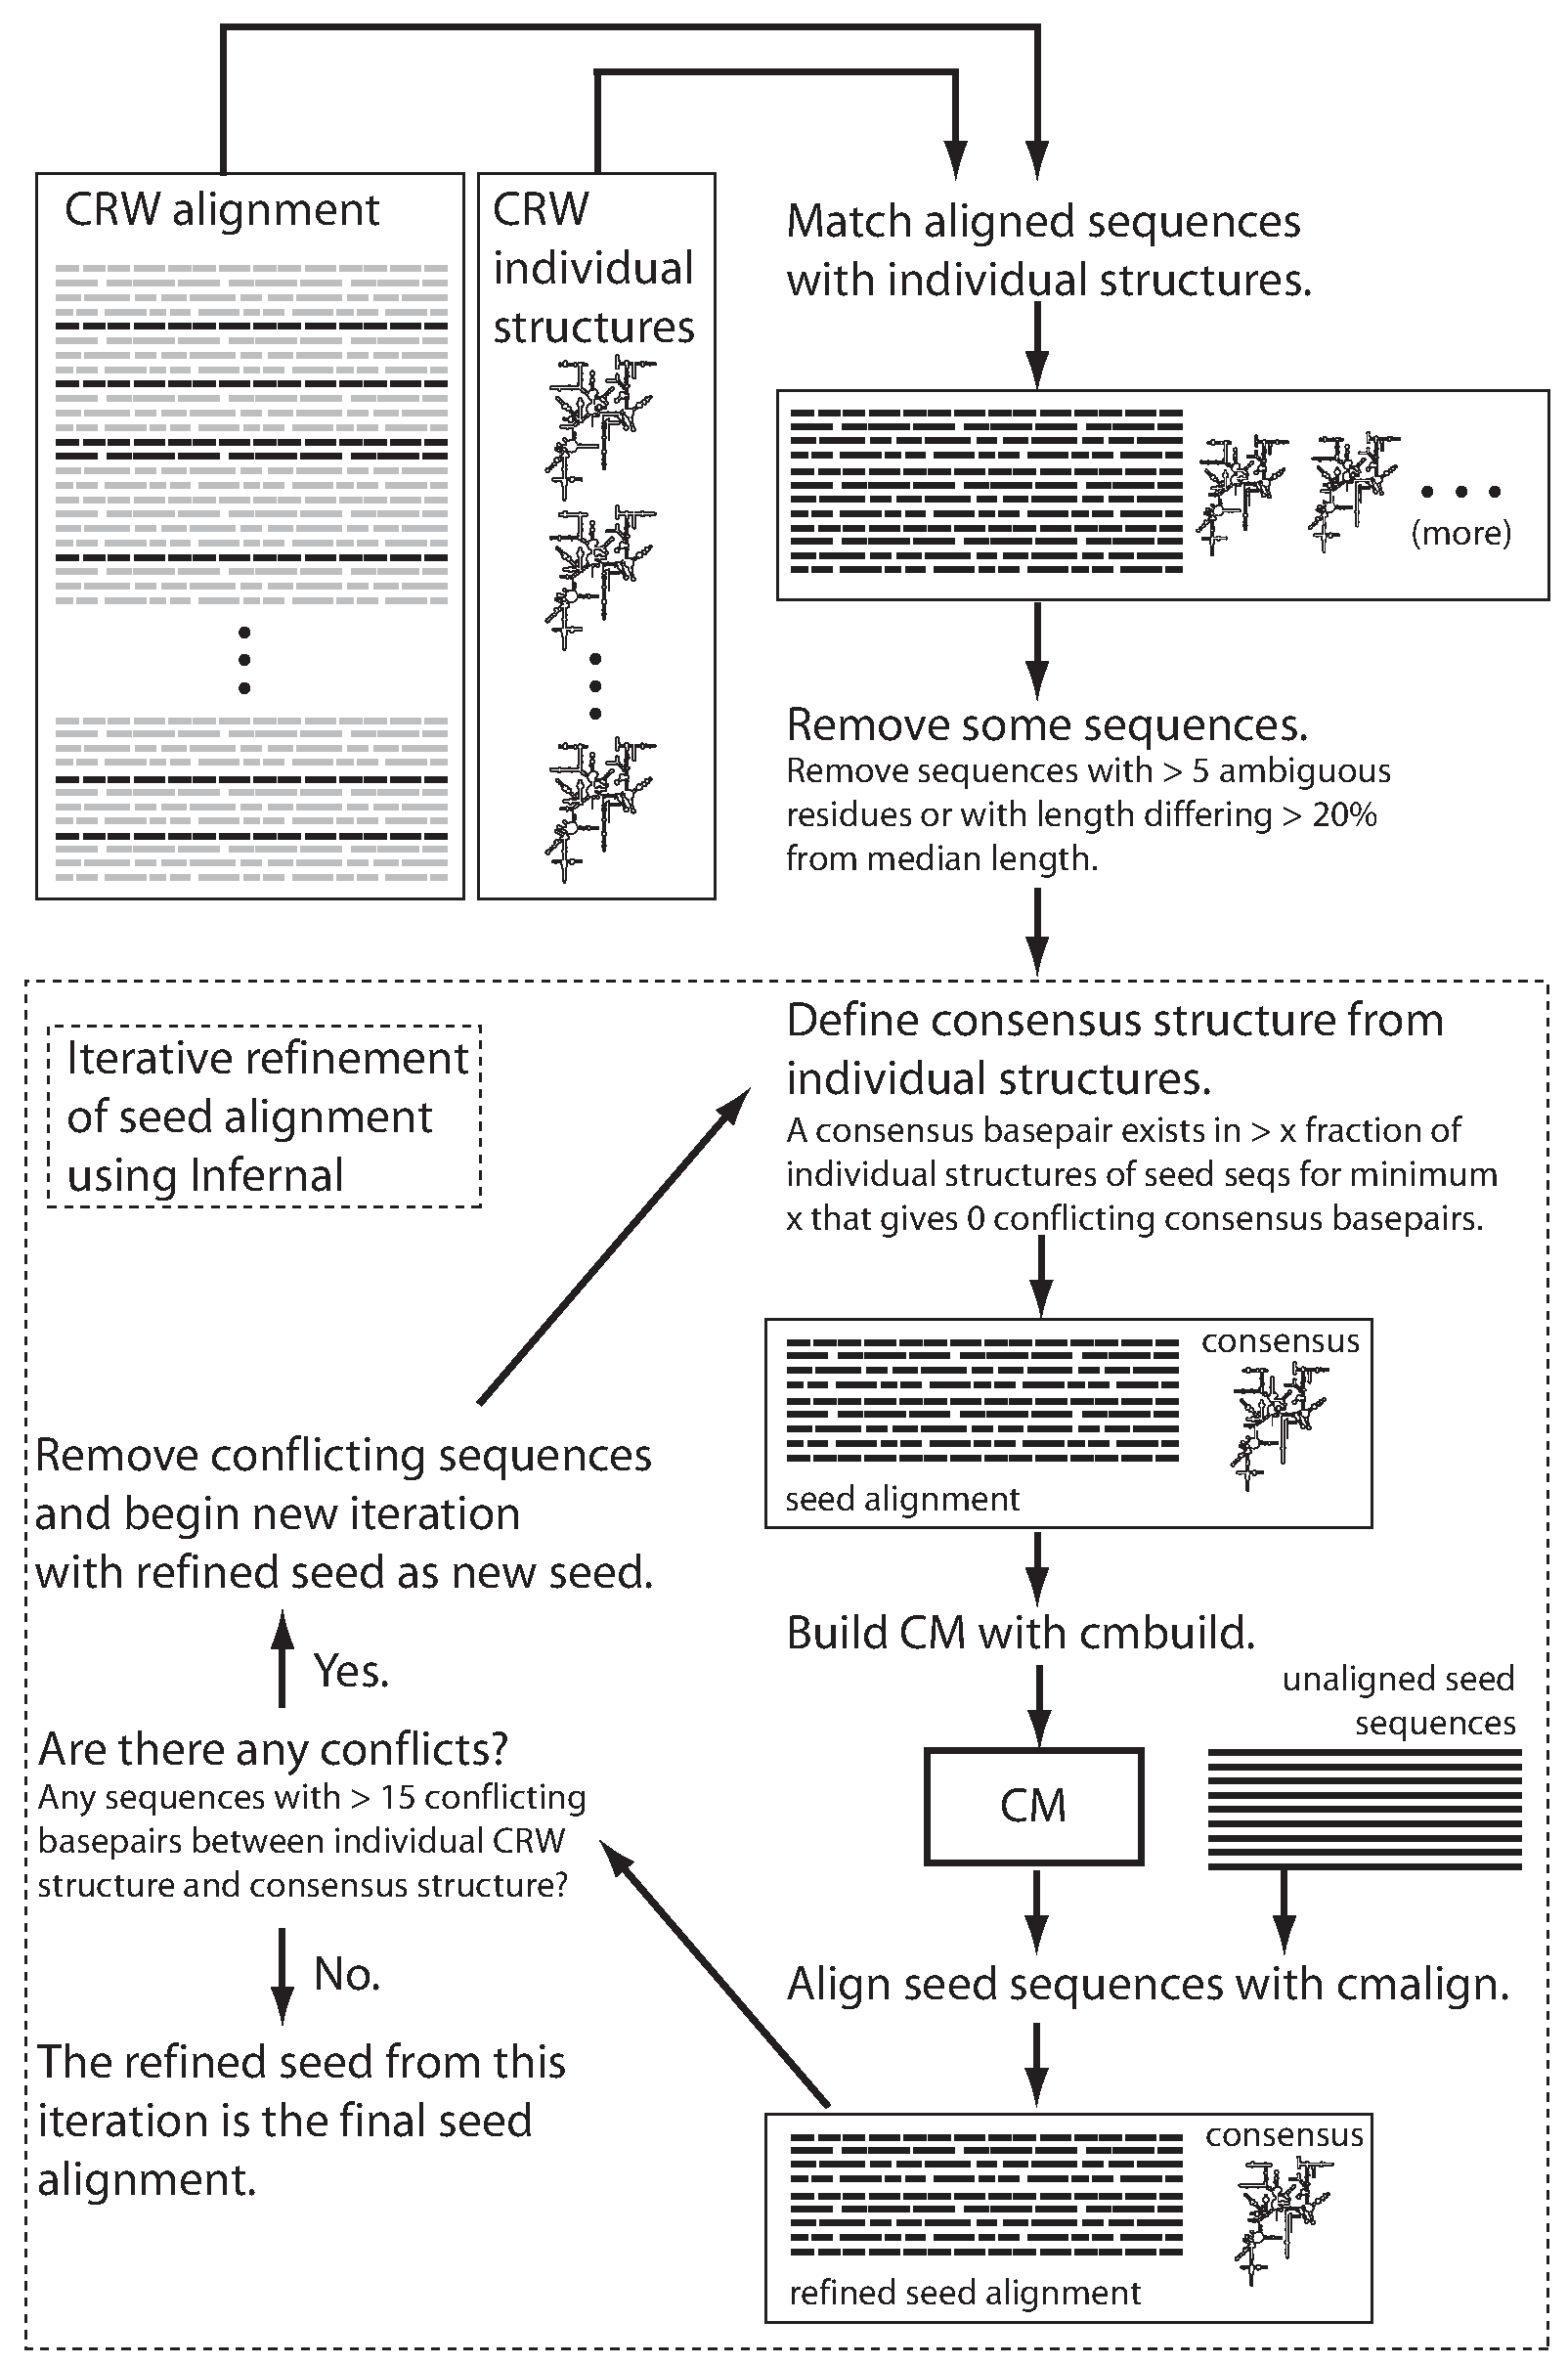
\includegraphics[height=6.9in]{Figures/crw2seed-schematic}
        \caption[The procedure for converting SSU alignments and
          individual structures from \db{crw} to seed alignments for
          SSU-ALIGN.]  {\textbf{The procedure for converting
            SSU alignments and individual structures from \db{crw} to seed
            alignments for SSU-ALIGN}. \db{crw} individual structures
          only exist for a small subset of the sequences from the \db{crw}
          alignments (the black sequences among the majority of gray
          ones). Each conversion step is explained
          in more detail in the text. 
          Figure~\ref{fig:conflict}
          demonstrates an example of conflicting basepairs. 
          Table~\ref{tbl:crw2seed} includes alignment
          statistics and number of sequences surviving each step for
          each of the three seed alignments derived from \db{crw}.}
  \end{center}
\label{fig:crw2seed}
\end{figure}

The first step was to extract the aligned sequences that matched to
the individual structures from the master alignments.  An individual
structure sequence $i$ and an aligned sequence $a$ qualified as match
if: $a$ and $i$ both had the same sequence accession, and the
unaligned sequence of $a$ was either identical to $i$ or an exact
subsequence of $i$.  Not all of the individual structures $i$ had a
matching aligned sequence $a$ per these criteria.  The number of
matches per alignment is shown below:

\begin{center}
\begin{tabular}{l|r|r|r}
%\begin{tabular}{lrrr}
             &               &            & \# of   \\ 
             & \# of aligned & \# of      & matches  \\ 
family       & sequences     & structures & (overlap) \\ \hline%& matches \\ \hline
archaea      &           132 &         25 &  23      \\%& 0.92 \\
bacteria     &          1266 &        231 &  95      \\%& 0.41 \\ 
%chloroplast  &           404 &         33 &  24      \\%& 0.73 \\ 
eukarya      &          1937 &        259 & 148      \\%& 0.57\\ 
%mitochondria &           899 &         96 &  80      \\%& 0.83 \\ 
\end{tabular}
\end{center}

This defines three sets of aligned sequences in which each sequence 
has its own predicted structure. CMs can only model well-nested
basepairing interactions, so all pseudoknotted basepairs
were removed from the individual structures. A well-nested structure
is a set of basepairs for which no two pairs between positions $i$:$j$
and $k$:$l$ exist such that $i<k<j<l$. I used the program
KNOTTED2NESTED.PY by \cite{Smit08} to remove
pseudoknots using the \texttt{-m OSP} option which maximizes the number
of basepairs in the resulting nested structure.
% more on if there are > 1 structure with identical # pairs?  see
% http://www.ibi.vu.nl/programs/k2nwww/static/method.html

From this set, any sequences with more than 5 ambiguous bases were
removed because ambiguous bases in a seed alignment inject noise into
the parameters of a CM (equation 1.4 of
\cite{Nawrocki09b}). Additionally, sequences less than 80\%, or more
than 120\% the median length of the alignment were removed\footnote{33
  eukaryotic sequences were less than 80\% the median length
  (table~\ref{tbl:crw2seed}). I plan to build an additional eukaryotic
  model of these shorter sequences for a future release of
  SSU-ALIGN}..

At this stage, basepairing \emph{conflicts} between the aligned
individual structures were identified. A conflict exists between two
basepairs in different structures, one between alignment columns
\emph{i} and \emph{j} and the other between columns \emph{k} and
\emph{l}, if $i = k$ and $j \neq l$, or $j = l$ and $i \neq k$.  An
example of two conflicting basepairs is shown in
Figure~\ref{fig:conflict}.  Conflicting basepairs are problematic
because a consensus basepair between columns $i$ and $j$ in a CM seed
alignment is assumed to exist (or be deleted) between the nucleotides in
$i$ and $j$ in \emph{all} sequences of the alignment. Columns involved
in conflicting basepairs violate this assumption by specifying that a
nucleotides in a single column is involved in different basepairs in
different sequences.

\begin{figure}[ht]
\ttfamily
\begin{center}
\begin{tabular}{ll}
%%%%%%%%%%%%%%%%%%%%%%%%%%%%%%
% Real example from original \db{crw} alignment (CRW matches stage) in
% Table crw2seed. 
% The original alignment file is:
% ~/notebook/9_0504_ssu_crw2ss_cons/final_conversion_redo_062909/bac/bac.0.indi.stk
                                          &           .........i....j.......  \\
00560::Xylella\_fastidiosa                &           GCAGGGGACCUUAGGGCCUUGU  \\ 
\#=GS 00560::Xylella\_fastidiosa SS       &           <<<<<<..<<....>>>>>>>>  \\
00018::Thermomicrobium\_roseum            &           GGCGCA--G-GCGAC-UGUGCU  \\
\#=GS 00018::Thermomicrobium\_roseum SS   &           <<<<<<..<.....>.>>>>>>  \\
                                          &           ........k.....l.......  \\
\end{tabular}
\rmfamily
        \caption[Example of conflicting basepairs between two aligned
          individual SSU structure predictions from CRW.]{
        \textbf{Example of conflicting basepairs between two aligned
          individual SSU structure predictions from CRW.}  The
        individual basepair between aligned columns $i$ and $j$ in
        \emph{Xylella fastidiosa} (sequence accession \texttt{M34115})
        conflicts with the \emph{Thermomicrobium roseum} (accession
        \texttt{AE003861}) basepair between columns $k$ and $l$ as
        defined in the text (because $i \neq k$ and $j = l$).}
\end{center}
\label{fig:conflict}
\end{figure}


Next, I removed conflicts using an iterative alignment refinement
procedure that eliminates sequences with more than 15 conflicts after
each iteration. The alignments at each stage are determined using a
CM\@. The initial consensus structure used to build the CM for the first
iteration was defined as the set of consensus base pairs between
alignment positions $i$ and $j$ that exist as paired in more than
\emph{x} fraction of the individual structures. The value for \emph{x}
was determined as the minimum value for which there were no
conflicting basepairs in the consensus set.

This provided me with an initial alignment that I then iteratively
refined using INFERNAL. Each iteration consists of a build
step, an alignment step, and a sequence removal step. First, a CM is
built from the current alignment (in iteration 1 this is a subset of
the \db{crw} alignment). Then all of the seed sequences are aligned to the
CM to generate a new alignment. The individual structures are mapped
onto the new alignment and a new consensus structure is derived as
described above.  Any sequence with more than 15 basepair conflicts
between its individual structure and the new consensus structure are
removed from the seed.  This procedure continues until 0 sequences are
removed in the final step. The alignment generated during the final
iteration became the seed alignment I used for SSU-ALIGN.

Table~\ref{tbl:crw2seed} lists the number of sequences removed at each
stage of the procedure and statistics on basepair conflicts. 
The three final seed alignments used to create the SSU-ALIGN 
models are summarized in Table~\ref{tbl:finalseeds}.


%%%%%%%%%%%%%%%%%%%%%%%%%%%%%%%%%%%%%%%%%%%%%%%%%%%%%%%%%%%%%%%
% crw2seed table
%%%%%%%%%%%%%%%%%%%%%%%%%%%%%%%%%%%%%%%%%%%%%%%%%%%%%%%%%%%%%%%
% original data is from 9_0507_ssu_crw2sscons_stk/00LOG on 06.29.09
\begin{table}[ht]
\begin{center}
  \small
  \begin{tabular}{llrrrrr|cccc}
% following table includes bp per seq and conflict bp per seq created with (local to MacBook):
% <[ssu]> perl crw2seed_tbl.pl crw2seed.tbl 
            &                       &      & cons   & \#          &
    avg \# & avg \# &        &       &       &     \\
            &                       & \#   & struct & cons        & indiv. & conflict&  \multicolumn{4}{c}{initial sequence removal} \\
      model & stage                 & seqs & $x$    & bps         & bps    & bps    &  total & ambig & short & long \\ \hline
            &                       &      &        &             &        &        &        &       &       &      \\ 
    archaea &           \db{crw} matches &   23 &  0.170 &         472 & 456.74 &   1.30 &   0    &     0 &     0 &    0 \\
    archaea &  post-initial removal &   23 &  0.170 &         472 & 456.74 &   1.30 &        &       &       &      \\
    archaea &        1st refinement &   23 &  0.130 &         474 & 456.74 &   0.52 &        &       &       &      \\
            &                       &      &        &             &        &        &        &       &       &      \\
   bacteria &           \db{crw} matches &   95 &  0.210 &         480 & 460.91 &   1.06 &   2    &     2 &     0 &    0 \\  
   bacteria &  post-initial removal &   93 &  0.200 &         480 & 460.82 &   1.05 &        &       &       &      \\
   bacteria &        1st refinement &   93 &  0.210 &         480 & 460.82 &   1.28 &        &       &       &      \\
            &                       &      &        &             &        &        &        &       &       &      \\
%chloroplast &           \db{crw} matches &   24 &  0.330 &         446 & 444.79 &   5.58 &   3    &     3 &     0 &    0 \\
%chloroplast &  post-initial removal &   21 &  0.230 &         450 & 444.48 &   6.24 &        &       &       &      \\
%chloroplast &        1st refinement &   21 &  0.190 &         450 & 444.48 &   7.24 &        &       &       &      \\
%chloroplast &        2nd refinement &   18 &  0.270 &         449 & 445.67 &   3.17 &        &       &       &      \\
%            &                       &      &        &             &        &        &        &       &       &      \\
    eukarya &           \db{crw} matches &  148 &  0.420 &         422 & 466.25 &  12.94 &  42    &    11 &    33 &    7 \\
    eukarya &  post-initial removal &  106 &  0.440 &         442 & 487.50 &  16.04 &        &       &       &      \\
    eukarya &        1st refinement &  106 &  0.410 &         448 & 487.50 &   8.71 &        &       &       &      \\
    eukarya &        2nd refinement &   89 &  0.440 &         448 & 487.73 &   5.49 &        &       &       &      \\
            &                       &      &        &             &        &        &        &       &       &      \\
%   metamito &           \db{crw} matches &   80 &  0.470 &         251 & 273.95 &   3.35 &  22    &     0 &     5 &   17 \\
%   metamito &  post-initial removal &   58 &  0.340 &         258 & 250.69 &   3.41 &        &       &       &      \\
%   metamito &        1st refinement &   58 &  0.340 &         258 & 250.69 &   4.83 &        &       &       &      \\
%   metamito &        2nd refinement &   55 &  0.360 &         256 & 252.64 &   3.71 &        &       &       &      \\
%            &                       &      &        &             &        &        &        &       &       &      \\
  \end{tabular}
\caption[Statistics on the conversion of CRW data to seed alignments for SSU-align.]
{\textbf{Statistics on the conversion of CRW data to seed alignments
    for SSU-align} For each of the three models, statistics for the
  alignments at each stage of the \db{crw} conversion process are
  shown. ``\db{crw} matches'' alignments are subsets of the
  \db{crw} alignments for matching sequences and individual
  structures. ``post-initial removal'' alignments have had sequences
  more than 120\% the median length (``long'' column), 
  less than 80\% the median length (``short'' column), or 
  with more than $5$ ambiguous bases (``ambig'' column) removed. 
  The remaining rows are for alignments following each round of the
  iterative refinement process using INFERNAL. More details on
  the \db{crw} conversion are in the text.}
\label{tbl:crw2seed}
\end{center}
\end{table}

\begin{table}[ht]
% stats from esl-alistat and cmbuild-1.0 on ssu5-0p1.stk
\begin{center}
\begin{tabular}{lrrrrrr} \hline
        &           &           &           &           & average   & average  \\
model   & number of & consensus & alignment & number of & sequence  & pairwise \\
name    & sequences & length    & length    & basepairs & length    & identity \\ \hline
archaea & 23        & 1508      & 1563      & 471       & 1485      & 81\%     \\
bacteria& 93        & 1582      & 1689      & 480       & 1527      & 80\%     \\
%chloroplast& 18     & 1514      & 1693      & 449       & 1492      & 85\%     \\
eukarya  & 89       & 1881      & 2652      & 448       & 1800      & 79\%     \\ 
%mitochondria  & 55       &  996      & 1127      & 256       & 957       & 76\%     \\
\end{tabular}
\caption[Statistics of the three seed alignments used by SSU-align.]
{\textbf{Statistics of the three seed alignments used by
    SSU-align.} These are the three alignments resulting from the
    CRW conversion depicted in Figure~\ref{fig:crw2seed} and
    described in the text.}
\label{tbl:finalseeds}
\end{center}
\end{table}

\newpage 

The final seed alignments are included in SSU-ALIGN package in
the \prog{seeds/} subdirectory as: \\ \prog{archaea-0p1.stk},
\prog{bacteria-0p1.stk}, and \prog{eukarya-0p1.stk}. Corresponding
unaligned FASTA files are also included, with a \prog{.fa} suffix
replacing \prog{.stk}. 

With the exception of the next page, the remainder of this section
includes 18 secondary structure diagrams displaying various statistics
per consensus column of the three seed alignments, with figure numbers
as indicated below. These structure diagrams can be created using
\prog{ssu-draw} with the following commands from the top-level
SSU-ALIGN directory:

\user{ssu-draw -a seeds/archaea-0p1.stk}

\user{ssu-draw -a seeds/bacteria-0p1.stk}

\user{ssu-draw -a seeds/eukarya-0p1.stk}

\vspace{0.2in}

\begin{center}
\begin{tabular}{r|l|l|l} \hline
statistic                        & archaea & bacteria & eukarya \\ \hline
consensus sequence               & Figure~\ref{fig:arcrf}  & Figure~\ref{fig:bacrf} & Figure~\ref{fig:eukrf} \\ 
information content              & Figure~\ref{fig:arcinfo} & Figure~\ref{fig:bacinfo} & Figure~\ref{fig:eukinfo} \\ 
mutual information               & Figure~\ref{fig:arcsinfo} & Figure~\ref{fig:bacsinfo} & Figure~\ref{fig:euksinfo} \\ 
frequency of deletions           & Figure~\ref{fig:arcdel} & Figure~\ref{fig:bacdel} & Figure~\ref{fig:eukdel} \\ 
frequency of insertions          & Figure~\ref{fig:arcifreq} & Figure~\ref{fig:bacifreq} & Figure~\ref{fig:eukifreq} \\ 
average insertion length         & Figure~\ref{fig:arciavglen} & Figure~\ref{fig:baciavglen} & Figure~\ref{fig:eukiavglen} \\ 
\end{tabular}
\end{center}

\subsection{Secondary structure diagrams summarizing the three models}

%%%%%%%%%%%%%%%%%%%%%%%%%%%%%%%%%%%%%%%%%%%%%%%%%%%%%%%%%%%%%%%%
%archaea
%%%%%%%%%%%%%%%%%%%%%%%%%%%%%%%%%%%%%%%%%%%%%%%%%%%%%%%%%%%%%%%%

\begin{figure}[hb]
\begin{center}
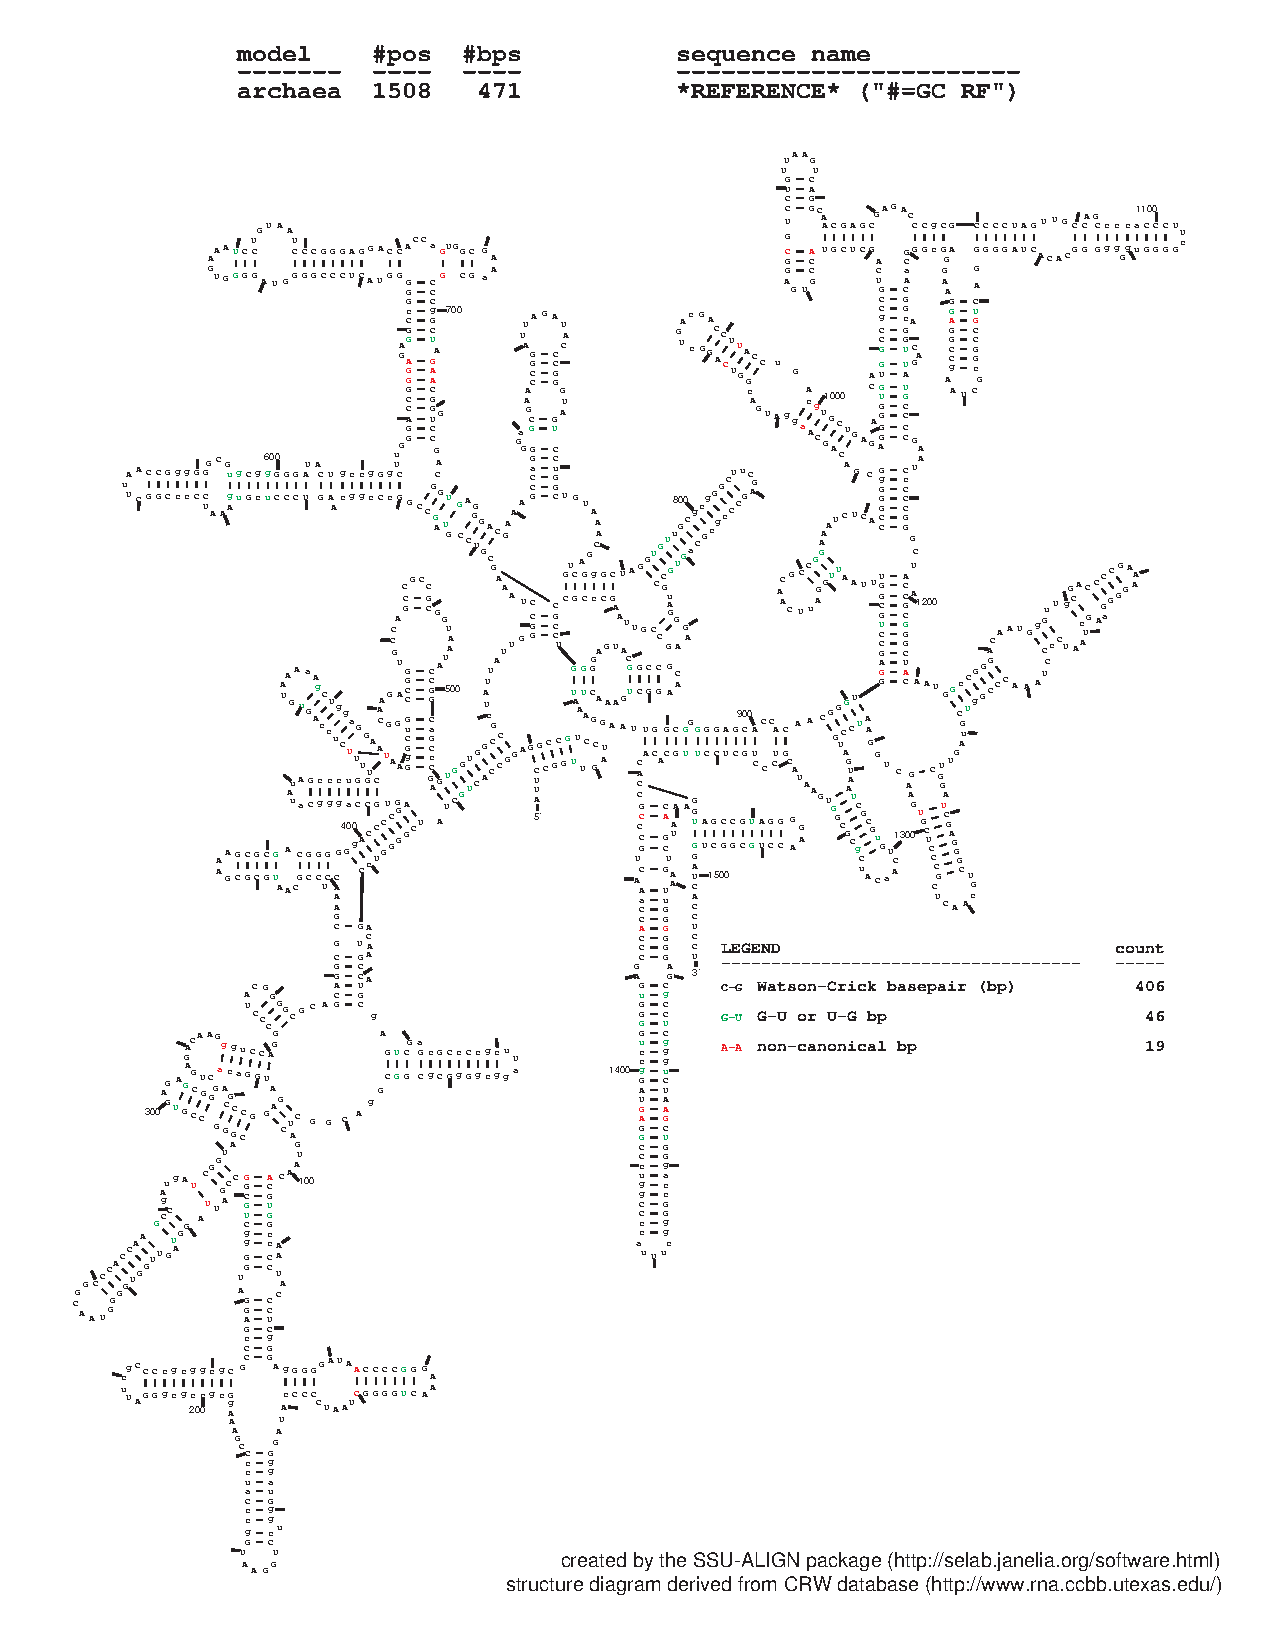
\includegraphics[width=5.64in]{Figures/archaea-0p1-rf}
\end{center}
\caption[Secondary structure diagram displaying the consensus sequence
  of the archaeal SSU model]{\textbf{Secondary structure diagram displaying the
  consensus sequence of the archaeal SSU model.} 
  This is the single sequence that the model 
  most closely represents and is the highest scoring possible
  sequence to the model. Uppercase nucleotides indicate highly conserved positions,
  and lowercase nucleotides indicate less well-conserved positions.
  This diagram was generated by the {\tt
  ssu-draw} program included in SSU-ALIGN}.
\label{fig:arcrf}
\end{figure}

\newpage 

\begin{figure}
\begin{center}
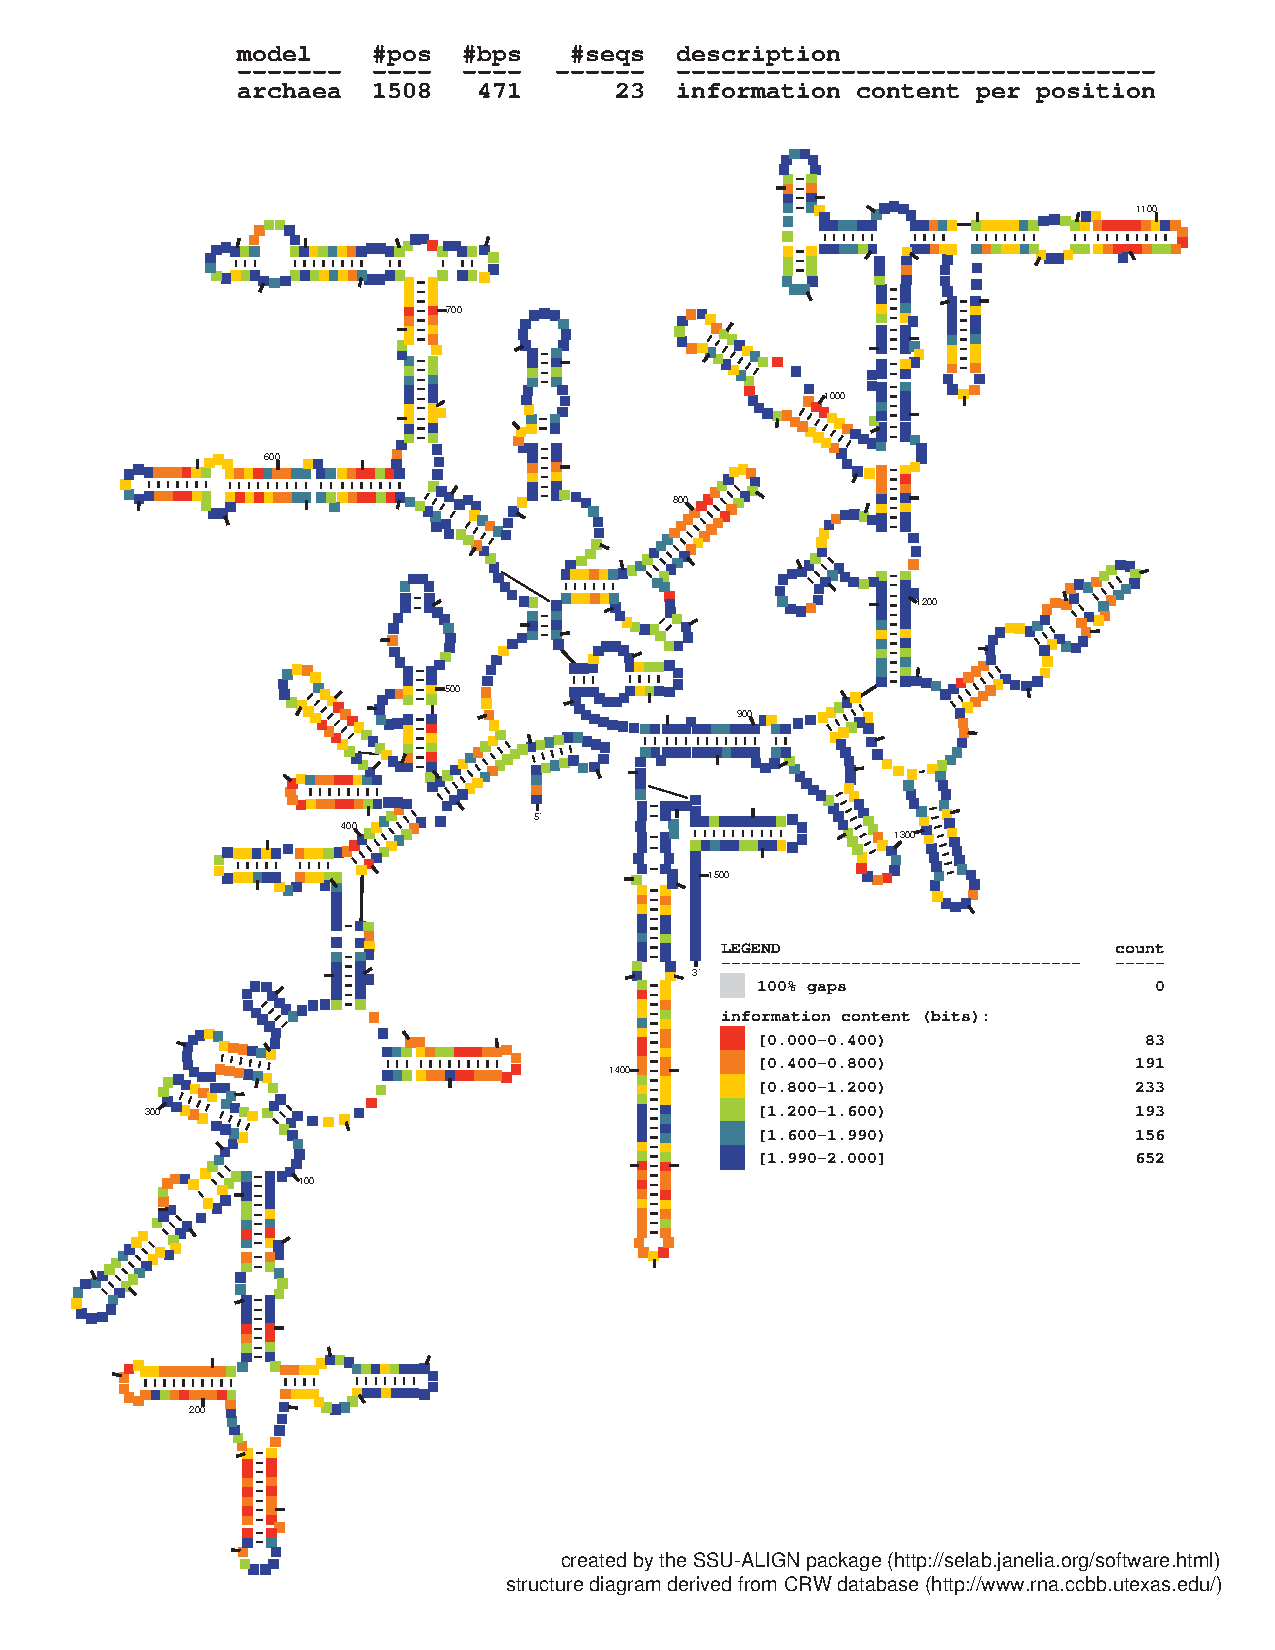
\includegraphics[width=5.64in]{Figures/archaea-0p1-info}
\end{center}
\caption[Secondary structure diagram displaying primary sequence
  information content per consensus position of the archaeal SSU seed
  alignment]{\textbf{Secondary structure diagram displaying primary
  sequence information content per consensus position of the archaeal SSU seed
  alignment.} Statistics correspond to the SSU-ALIGN seed
  alignment derived from the \db{crw} database \cite{CannoneGutell02}
  as described in the text. This diagram was generated by the {\tt
  ssu-draw} program included in SSU-ALIGN}.
\label{fig:arcinfo}
\end{figure}

\newpage 

\begin{figure}
\begin{center}
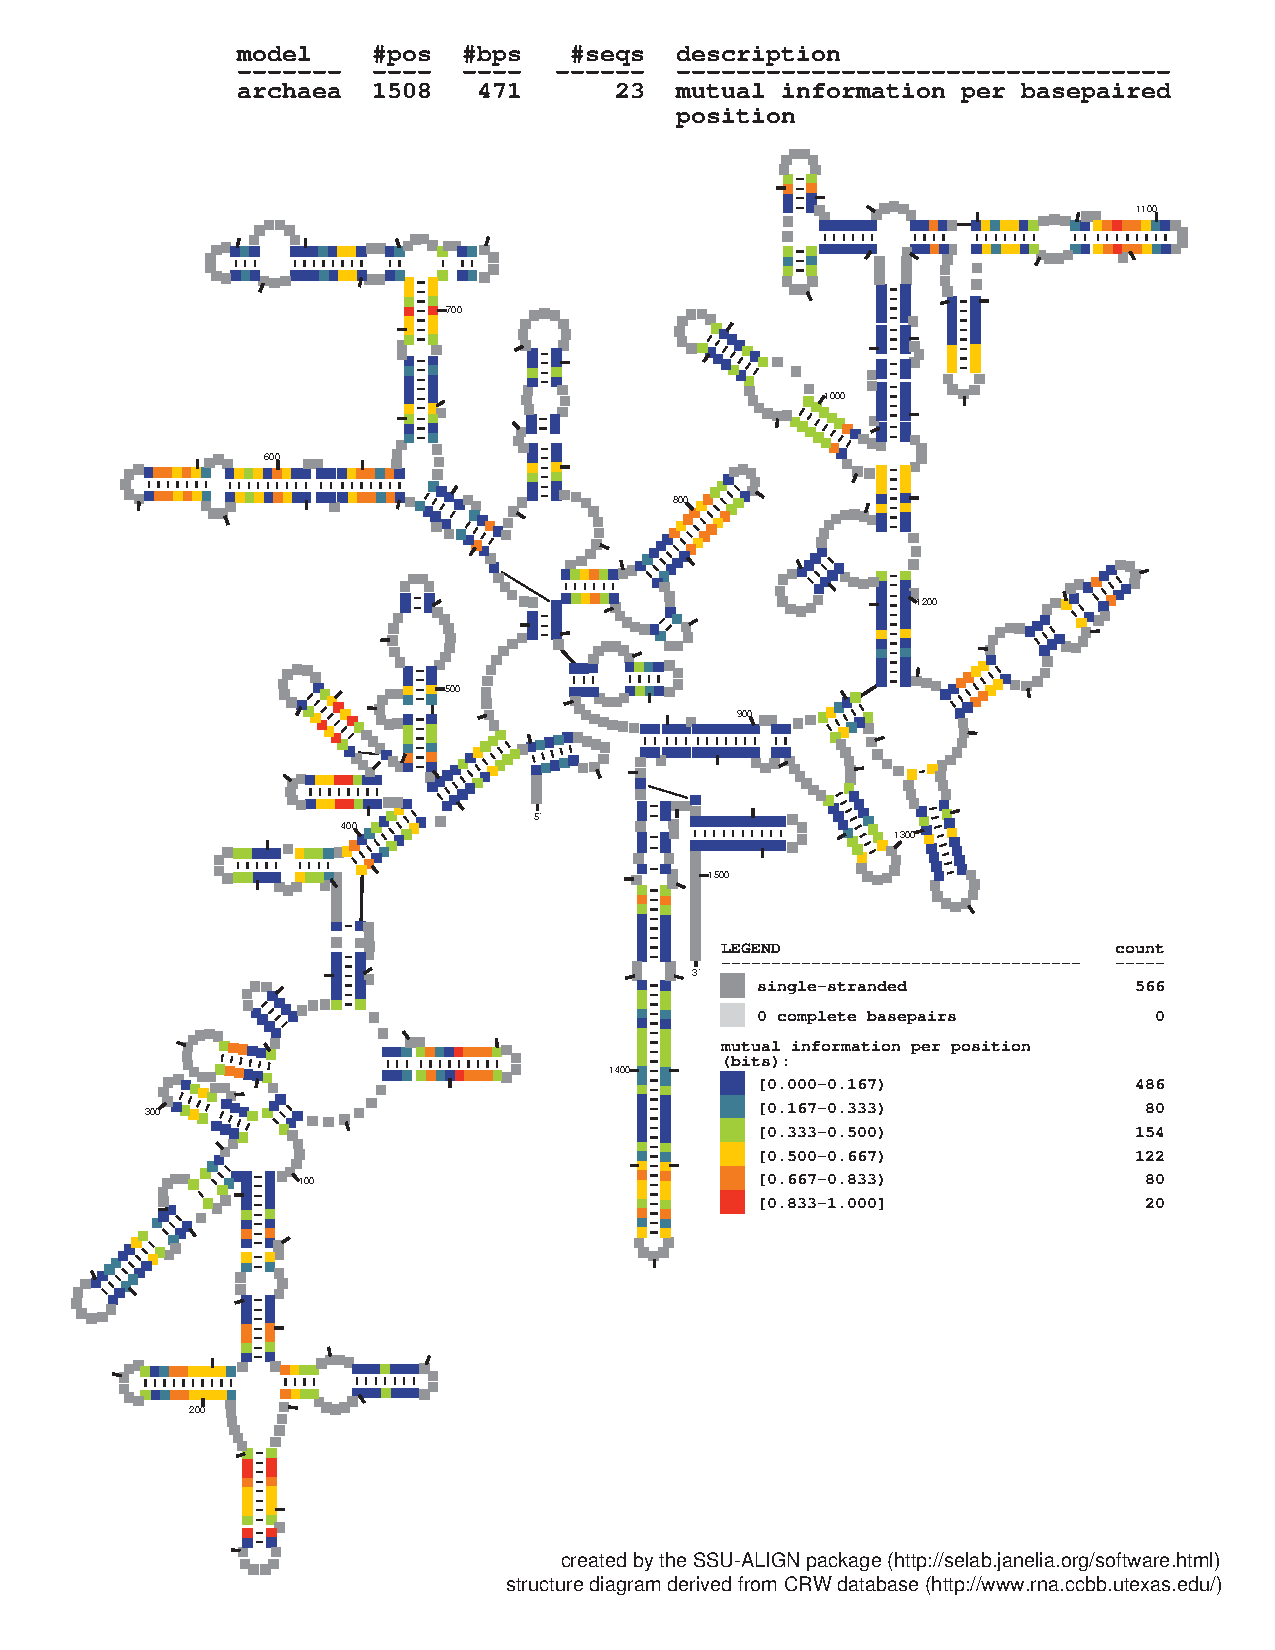
\includegraphics[width=5.64in]{Figures/archaea-0p1-mutinfo}
\end{center}
\caption[Secondary structure diagram displaying extra information 
  from conserved structure per consensus position of the archaeal SSU seed
  alignment]{\textbf{Secondary structure diagram displaying extra
  information from conserved structure per consensus position of the archaeal SSU seed
  alignment.} Statistics correspond to the SSU-ALIGN seed
  alignment derived from the \db{crw} database \cite{CannoneGutell02}
  as described in the text. This diagram was generated by the {\tt
  ssu-draw} program included in SSU-ALIGN}.
\label{fig:arcsinfo}
\end{figure}

\newpage 

\begin{figure}
\begin{center}
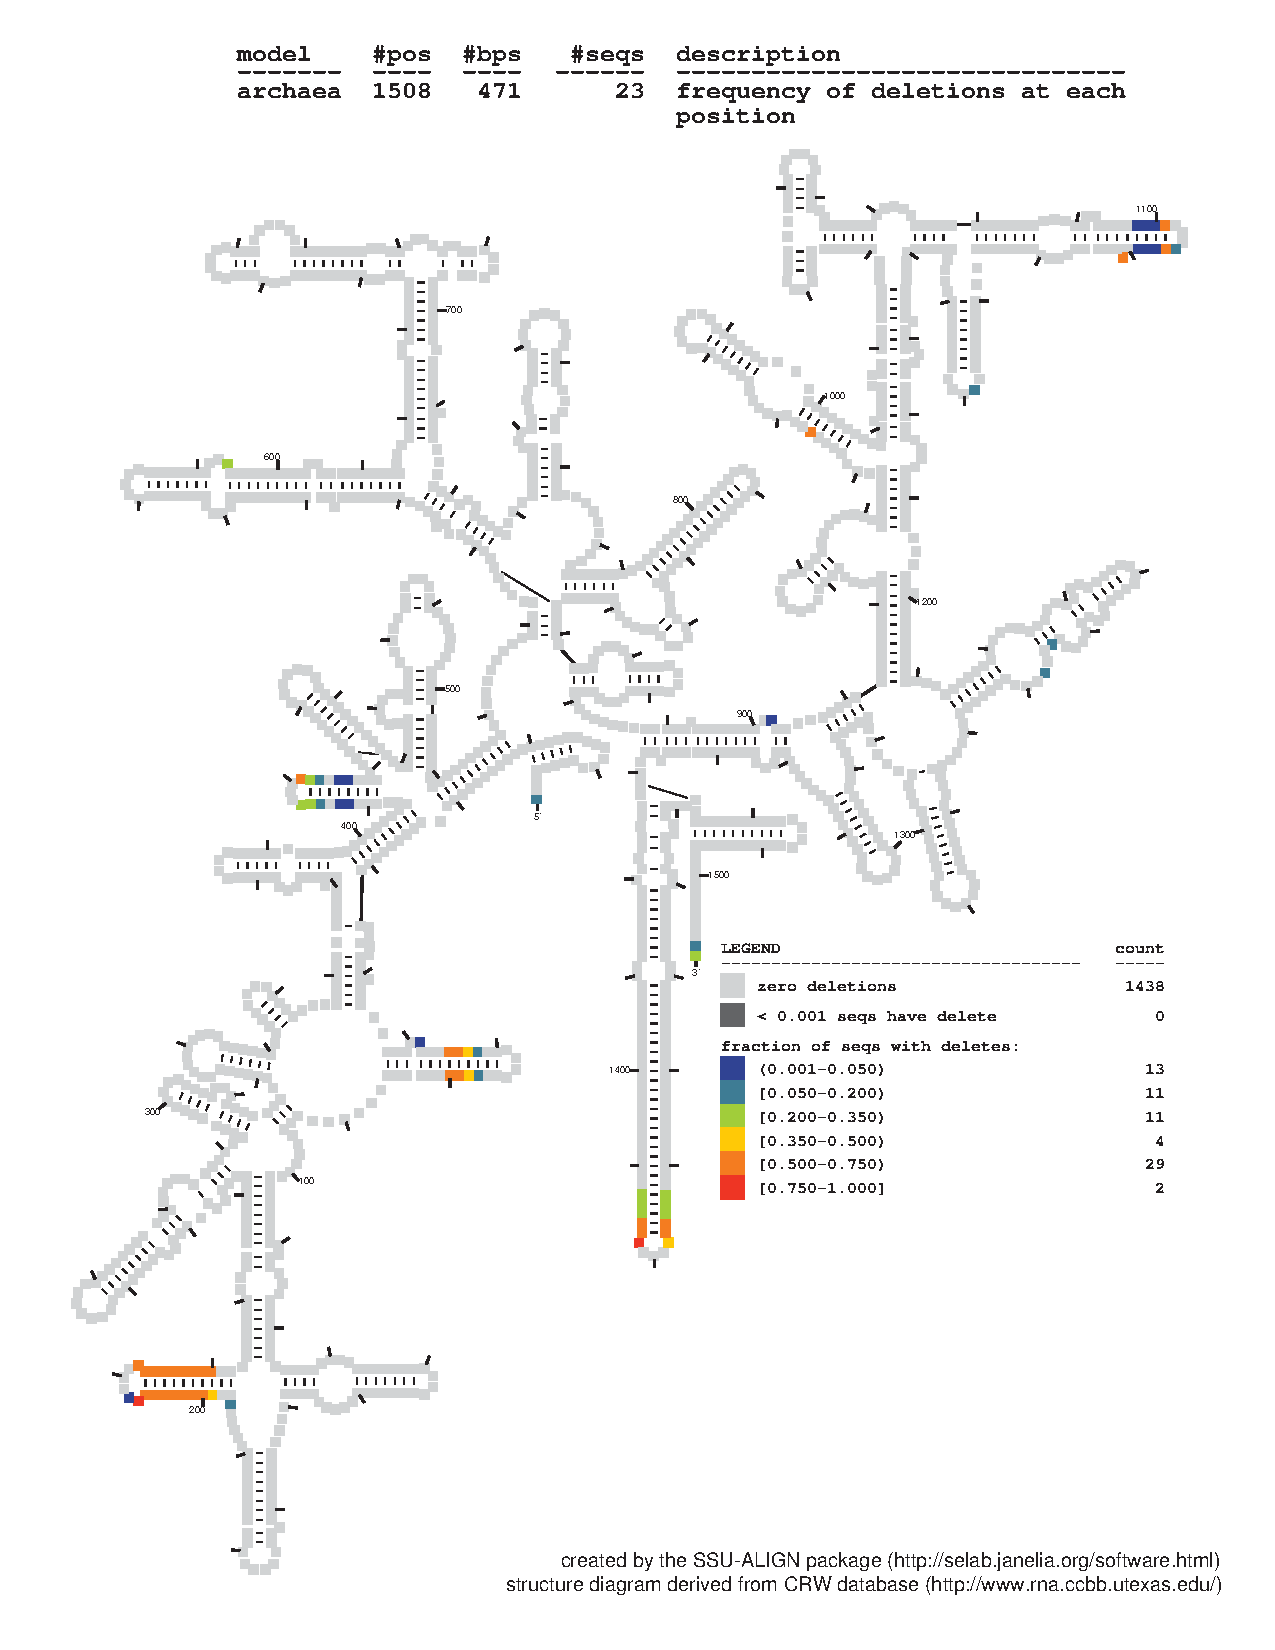
\includegraphics[width=5.64in]{Figures/archaea-0p1-dall}
\end{center}
\caption[Secondary structure diagram displaying frequency of deletions
  per consensus position of the archaeal SSU seed
  alignment]{\textbf{Secondary structure diagram displaying frequency 
  of deletions per consensus position of the archaeal SSU seed
  alignment.} Statistics correspond to the SSU-ALIGN seed
  alignment derived from the \db{crw} database \cite{CannoneGutell02}
  as described in the text. This diagram was generated by the {\tt
  ssu-draw} program included in SSU-ALIGN}.
\label{fig:arcdel}
\end{figure}

\newpage 

\begin{figure}
\begin{center}
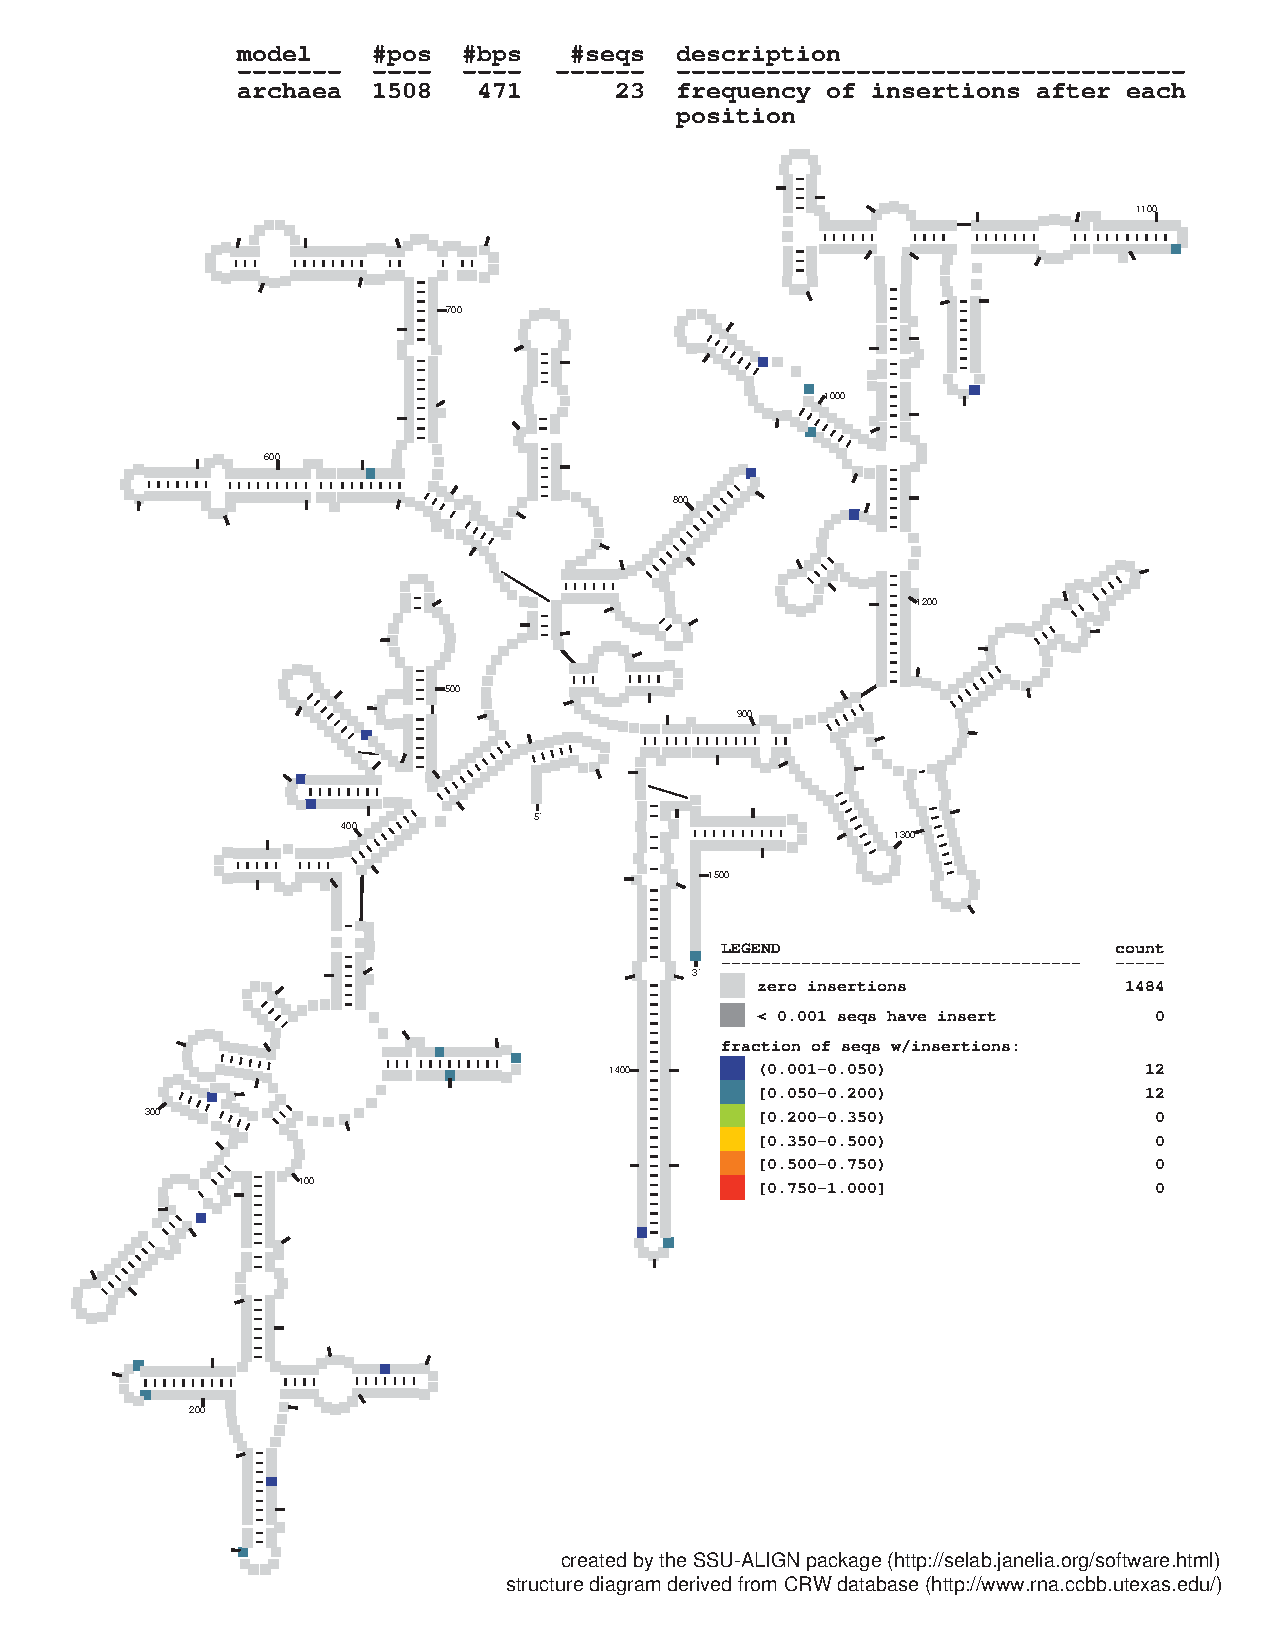
\includegraphics[width=5.64in]{Figures/archaea-0p1-ifreq}
\end{center}
\caption[Secondary structure diagram displaying frequency of insertions
  after each consensus position in the archaeal SSU seed
  alignment]{\textbf{Secondary structure diagram displaying frequency
  of insertions after each consensus position in the archaeal SSU seed
  alignment.} Statistics correspond to the SSU-ALIGN seed
  alignment derived from the \db{crw} database \cite{CannoneGutell02}
  as described in the text. This diagram was generated by the {\tt
  ssu-draw} program included in SSU-ALIGN}.
\label{fig:arcifreq}
\end{figure}

\newpage 

\begin{figure}
\begin{center}
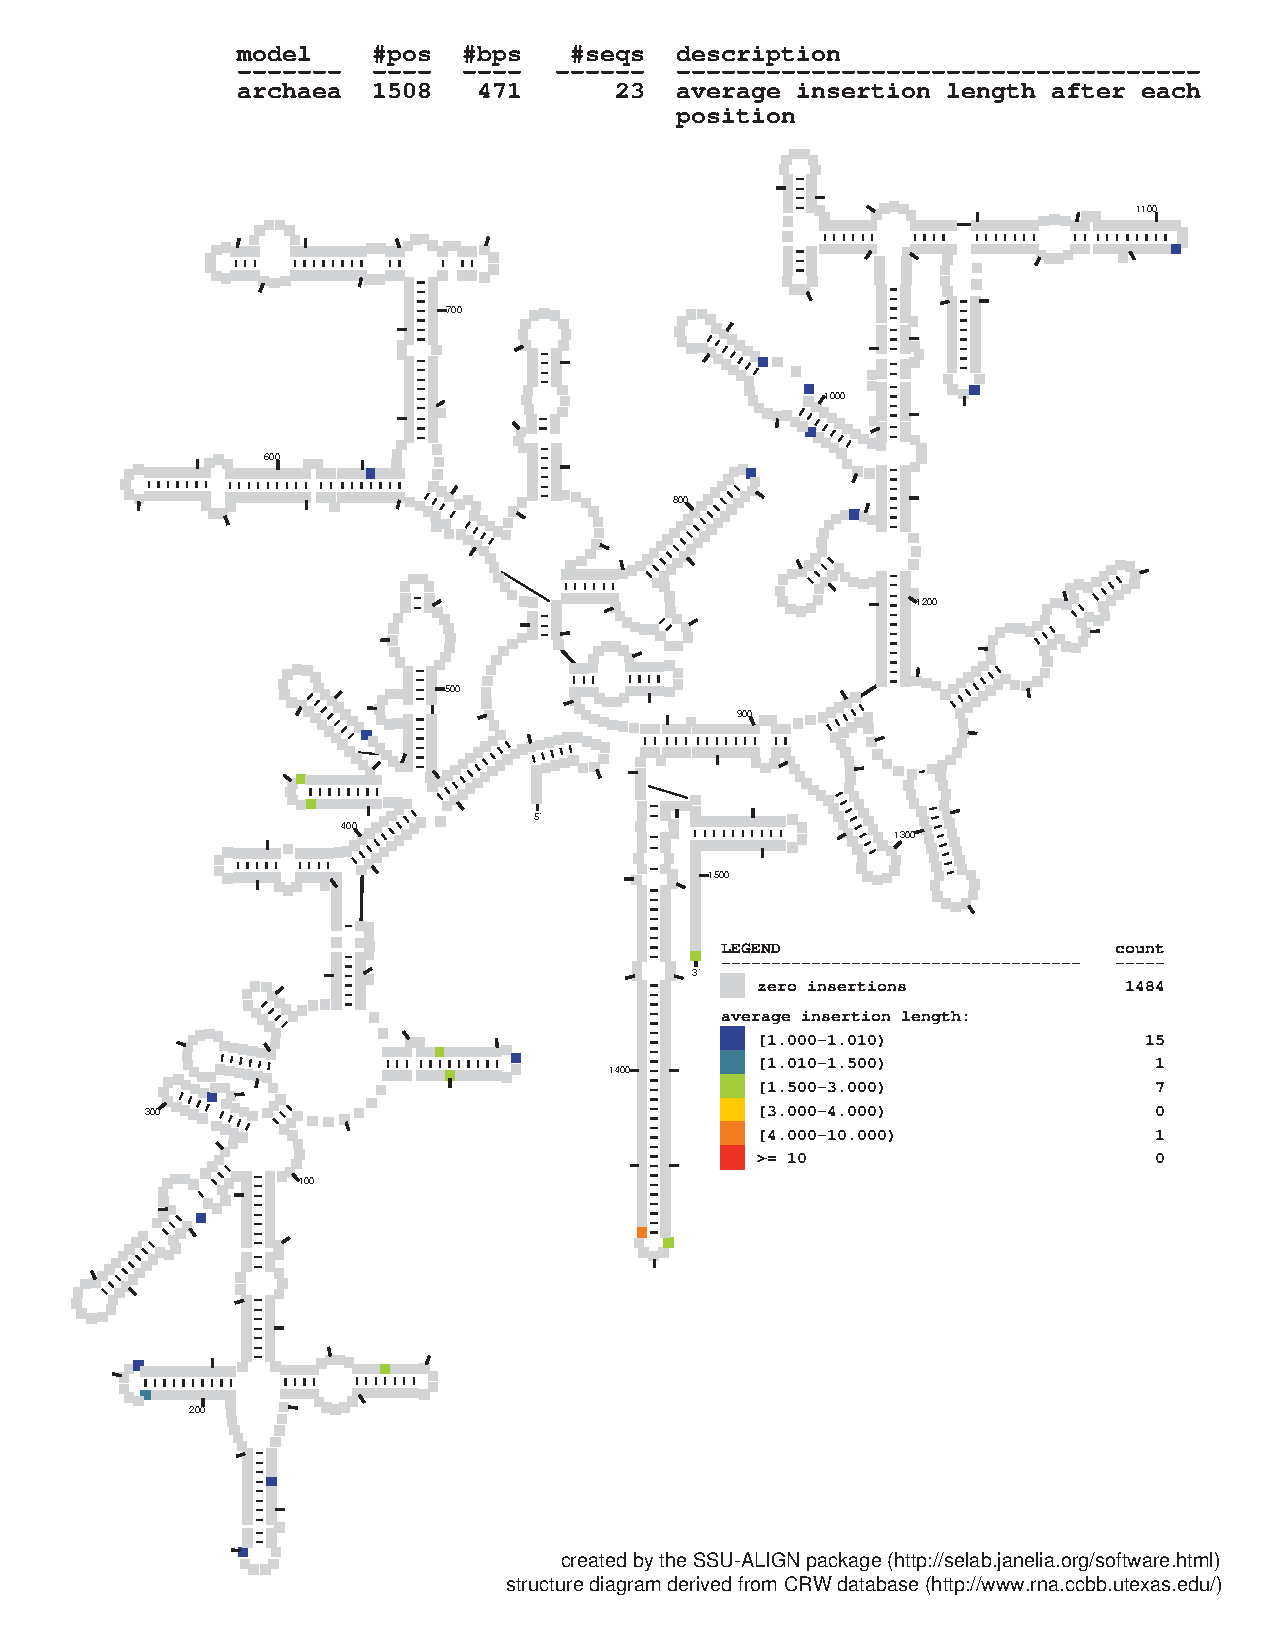
\includegraphics[width=5.64in]{Figures/archaea-0p1-iavglen}
\end{center}
\caption[Secondary structure diagram displaying average length of insertions
  after each consensus position in the archaeal SSU seed
  alignment]{\textbf{Secondary structure diagram displaying average
    length of insertions after each consensus position in the archaeal SSU seed
  alignment.} Statistics correspond to the SSU-ALIGN seed
  alignment derived from the \db{crw} database \cite{CannoneGutell02}
  as described in the text. This diagram was generated by the {\tt
  ssu-draw} program included in SSU-ALIGN}.
\label{fig:arciavglen}
\end{figure}


%%%%%%%%%%%%%%%%%%%%%%%%%%%%%%%%%%%%%%%%%%%%%%%%%%%%%%%%%%%%%%%%
%bacteria
%%%%%%%%%%%%%%%%%%%%%%%%%%%%%%%%%%%%%%%%%%%%%%%%%%%%%%%%%%%%%%%%
\newpage 

\begin{figure}
\begin{center}
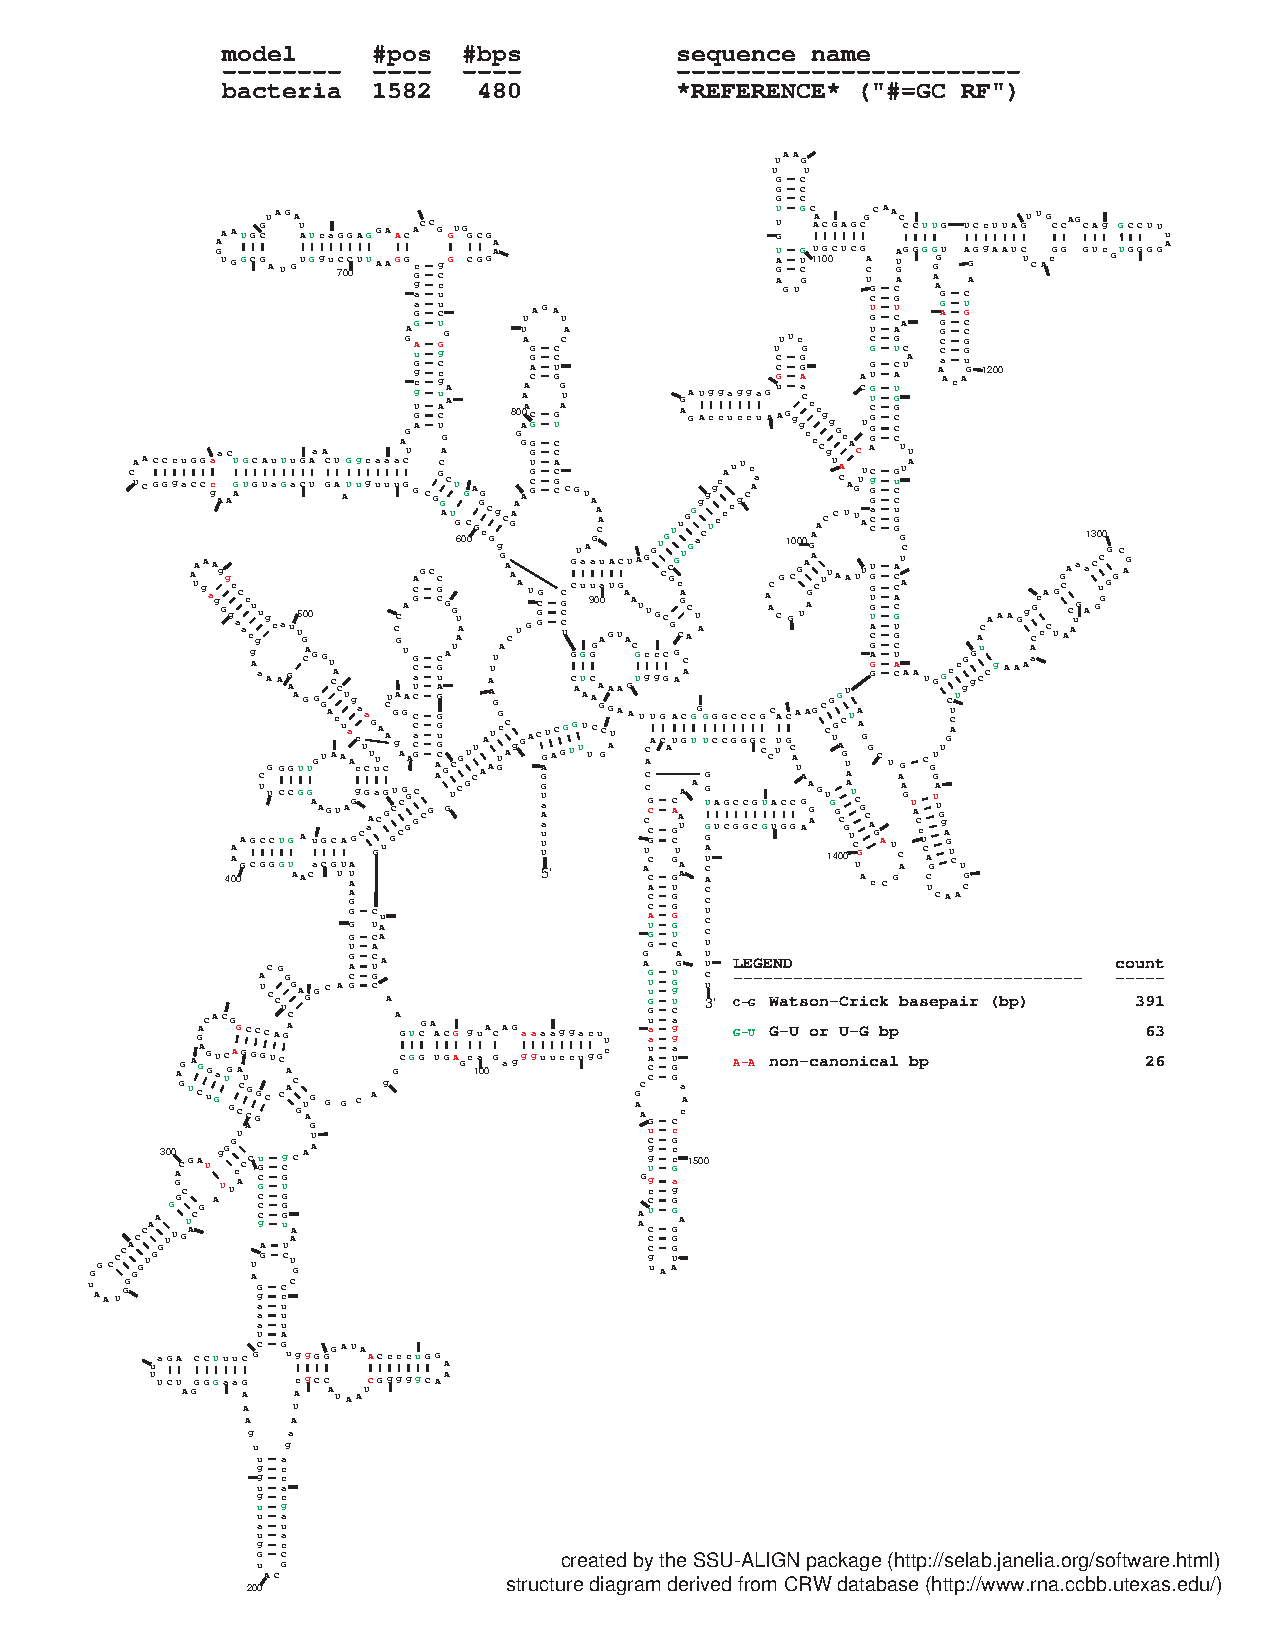
\includegraphics[width=5.64in]{Figures/bacteria-0p1-rf}
\end{center}
\caption[Secondary structure diagram displaying the consensus sequence
  of the bacterial SSU model]{\textbf{Secondary structure diagram displaying the
  consensus sequence of the bacterial SSU model.} 
  This is the single sequence that the model 
  most closely represents, and is the highest scoring possible
  sequence to the model. Uppercase nucleotides indicate highly conserved positions,
  and lowercase nucleotides indicate less well-conserved positions.
  This diagram was generated by the {\tt
  ssu-draw} program included in SSU-ALIGN}.
\label{fig:bacrf}
\end{figure}

\newpage 

\begin{figure}
\begin{center}
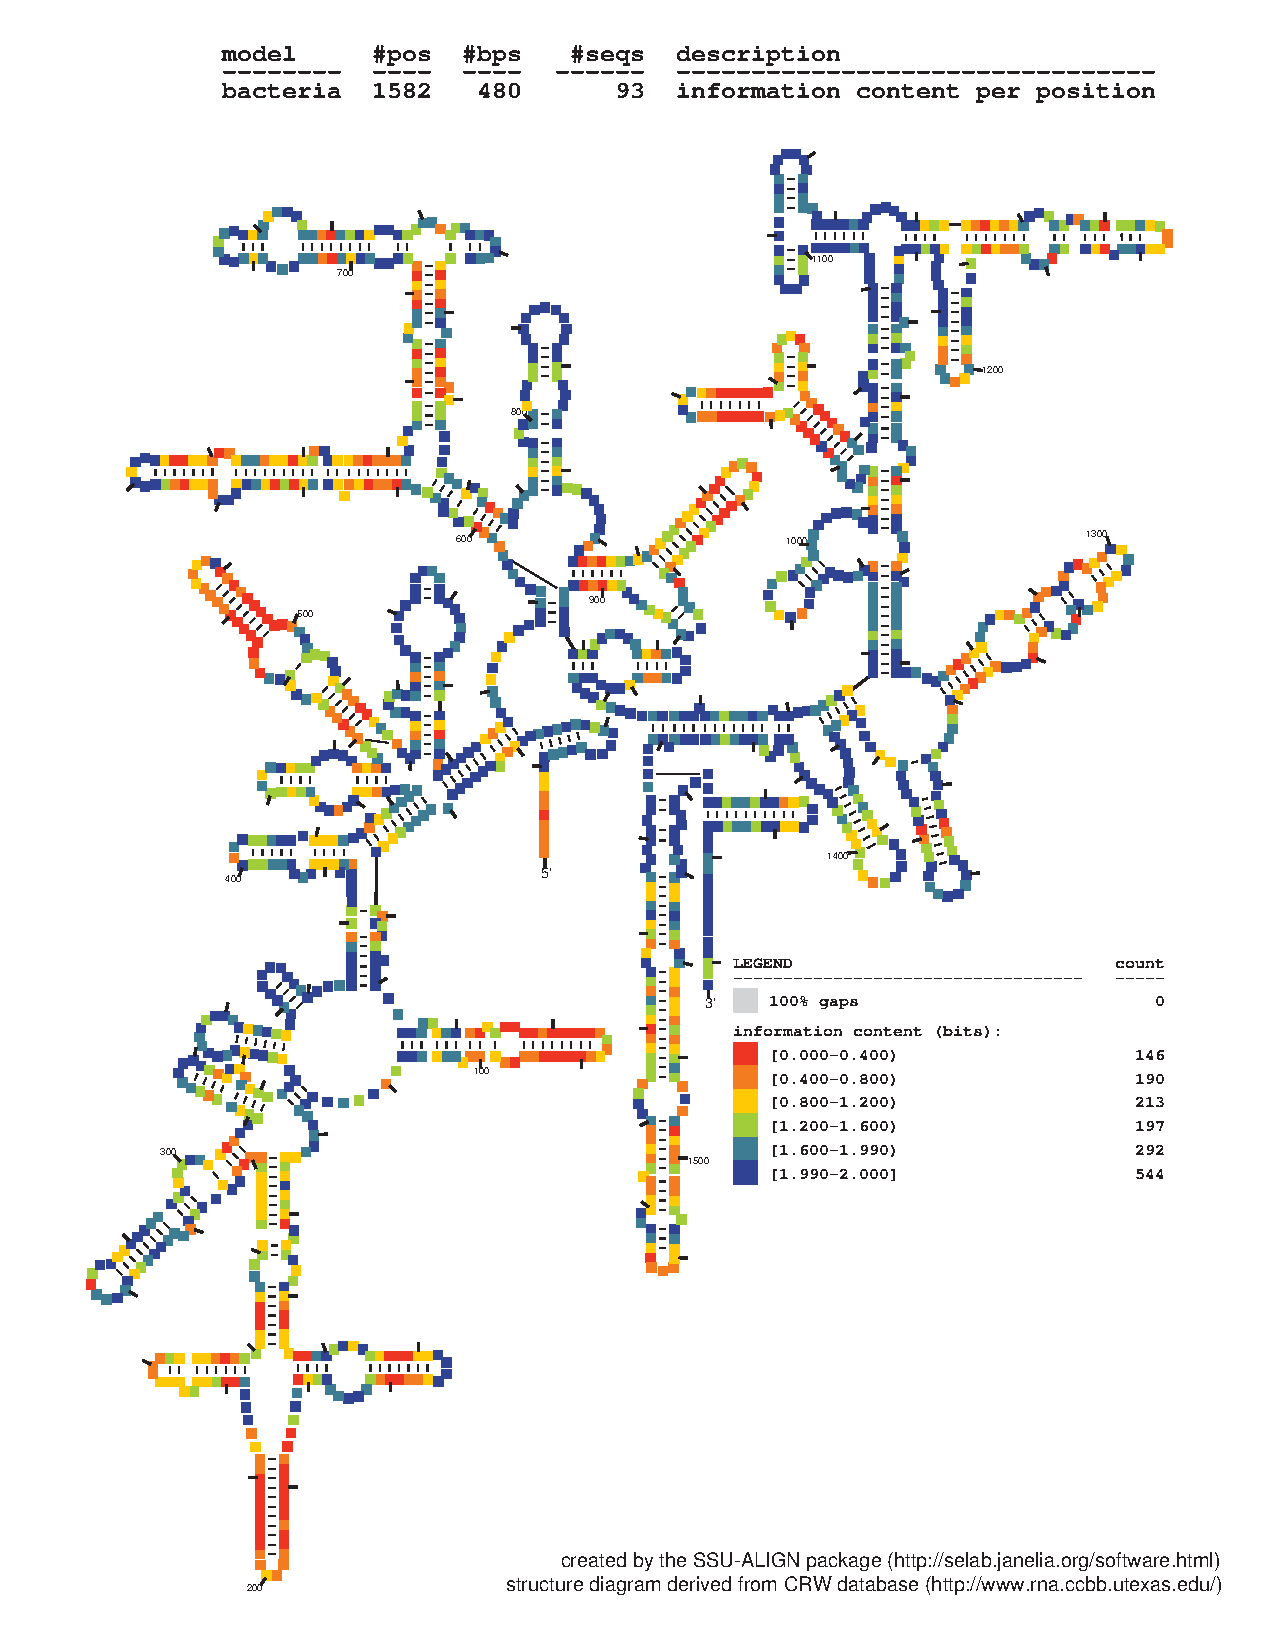
\includegraphics[width=5.64in]{Figures/bacteria-0p1-info}
\end{center}
\caption[Secondary structure diagram displaying primary sequence
  information content per consensus position of the bacterial SSU seed
  alignment]{\textbf{Secondary structure diagram displaying primary
  sequence information content per consensus position of the bacterial SSU seed
  alignment.} Statistics correspond to the SSU-ALIGN seed
  alignment derived from the \db{crw} database \cite{CannoneGutell02}
  as described in the text. This diagram was generated by the {\tt
  ssu-draw} program included in SSU-ALIGN}.
\label{fig:bacinfo}
\end{figure}

\newpage 

\begin{figure}
\begin{center}
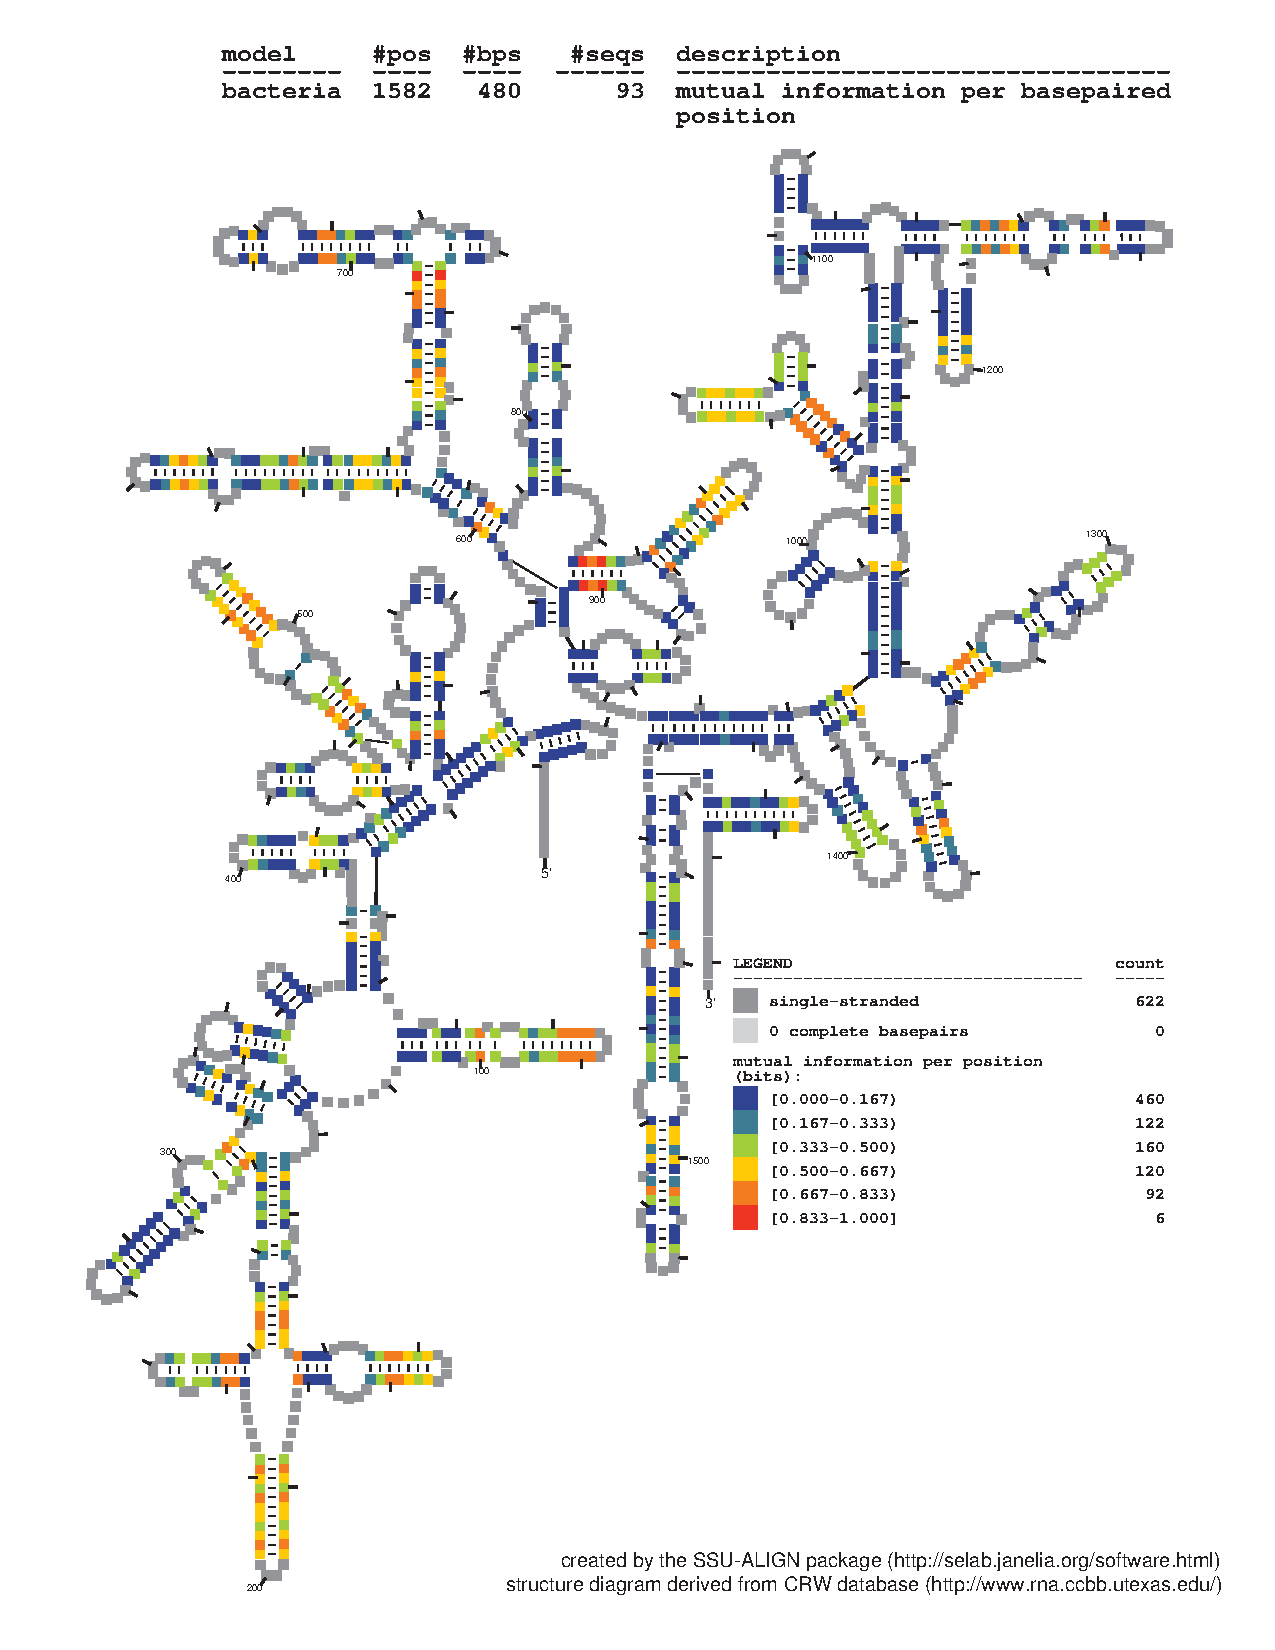
\includegraphics[width=5.64in]{Figures/bacteria-0p1-mutinfo}
\end{center}
\caption[Secondary structure diagram displaying extra information 
  from conserved structure per consensus position of the bacterial SSU seed
  alignment]{\textbf{Secondary structure diagram displaying extra
  information from conserved structure per consensus position of the bacterial SSU seed
  alignment.} Statistics correspond to the SSU-ALIGN seed
  alignment derived from the \db{crw} database \cite{CannoneGutell02}
  as described in the text. This diagram was generated by the {\tt
  ssu-draw} program included in SSU-ALIGN}.
\label{fig:bacsinfo}
\end{figure}

\newpage 

\begin{figure}
\begin{center}
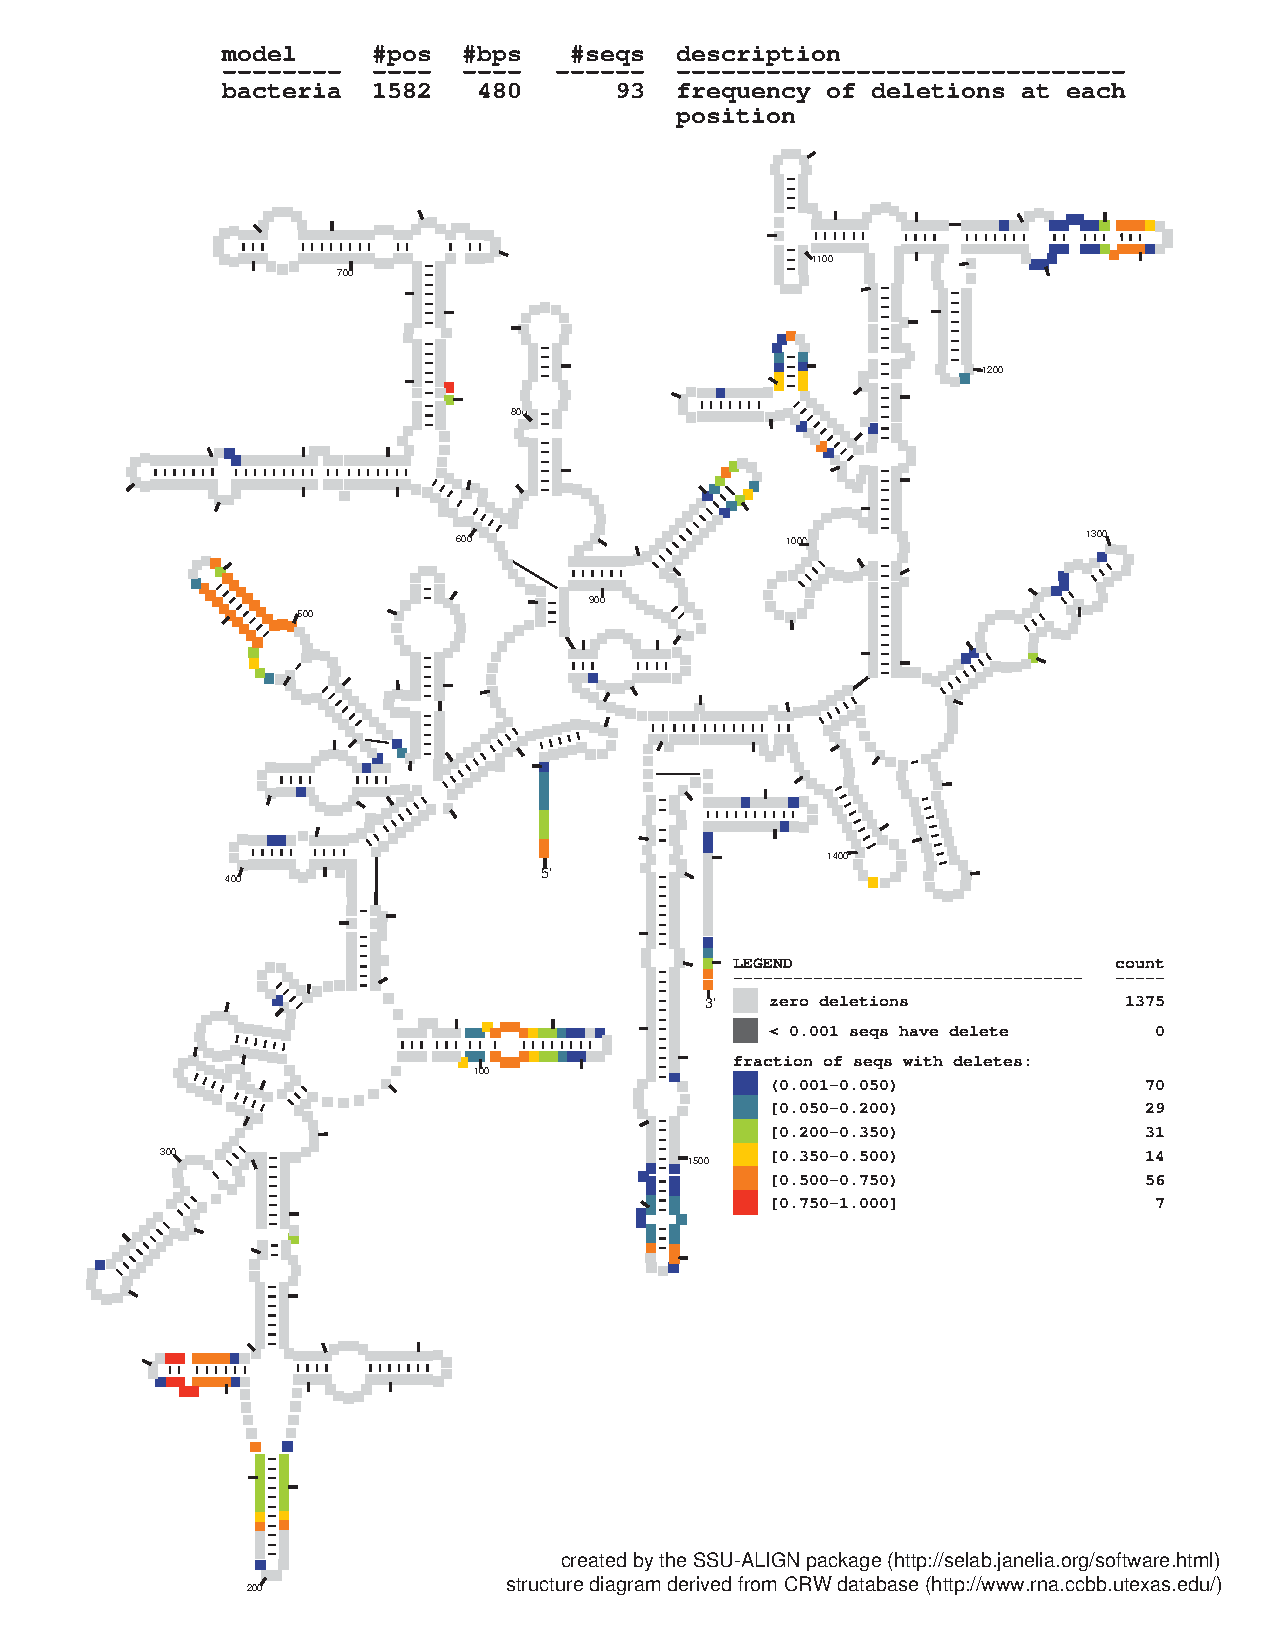
\includegraphics[width=5.64in]{Figures/bacteria-0p1-dall}
\end{center}
\caption[Secondary structure diagram displaying frequency of deletions
  per consensus position of the bacterial SSU seed
  alignment]{\textbf{Secondary structure diagram displaying frequency 
  of deletions per consensus position of the bacterial SSU seed
  alignment.} Statistics correspond to the SSU-ALIGN seed
  alignment derived from the \db{crw} database \cite{CannoneGutell02}
  as described in the text. This diagram was generated by the {\tt
  ssu-draw} program included in SSU-ALIGN}.
\label{fig:bacdel}
\end{figure}

\newpage 

\begin{figure}
\begin{center}
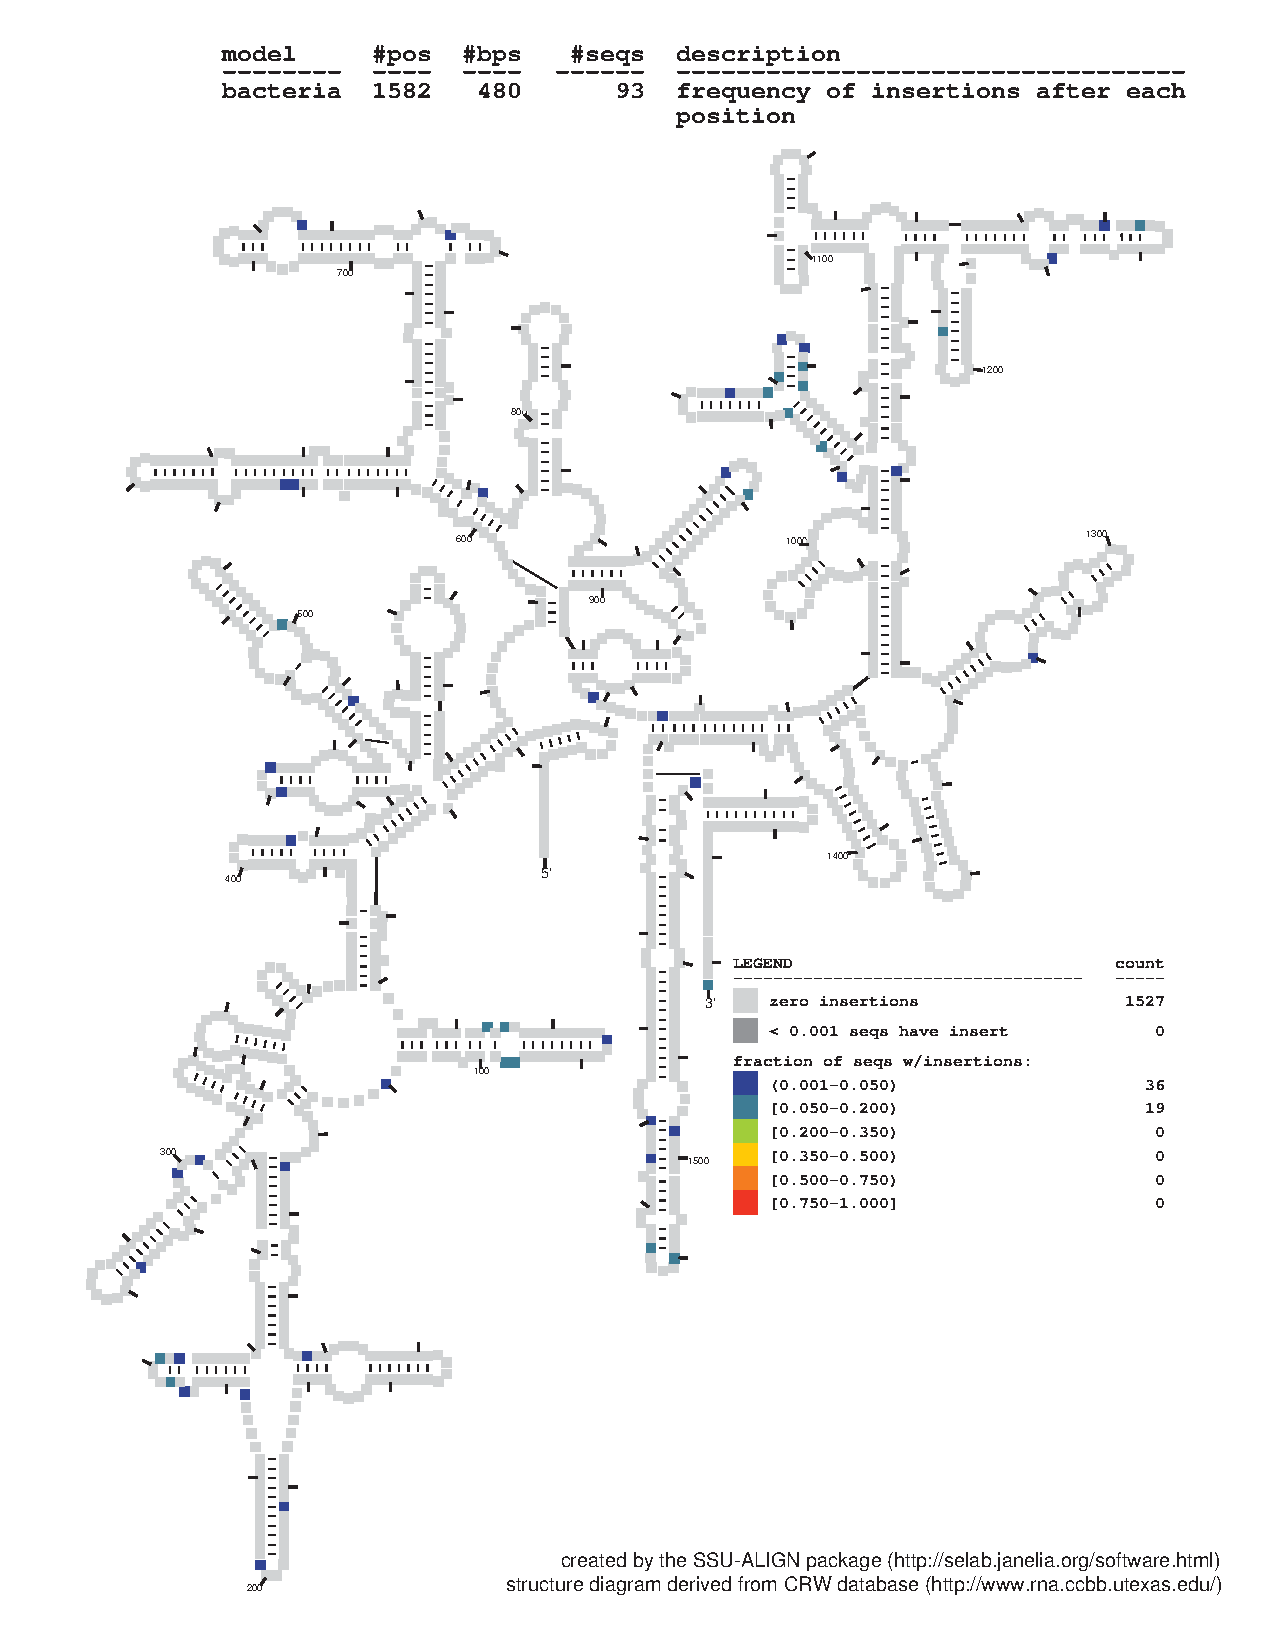
\includegraphics[width=5.64in]{Figures/bacteria-0p1-ifreq}
\end{center}
\caption[Secondary structure diagram displaying frequency of insertions
  after each consensus position in the bacterial SSU seed
  alignment]{\textbf{Secondary structure diagram displaying frequency
  of insertions after each consensus position in the bacterial SSU seed
  alignment.} Statistics correspond to the SSU-ALIGN seed
  alignment derived from the \db{crw} database \cite{CannoneGutell02}
  as described in the text. This diagram was generated by the {\tt
  ssu-draw} program included in SSU-ALIGN}.
\label{fig:bacifreq}
\end{figure}

\newpage 

\begin{figure}
\begin{center}
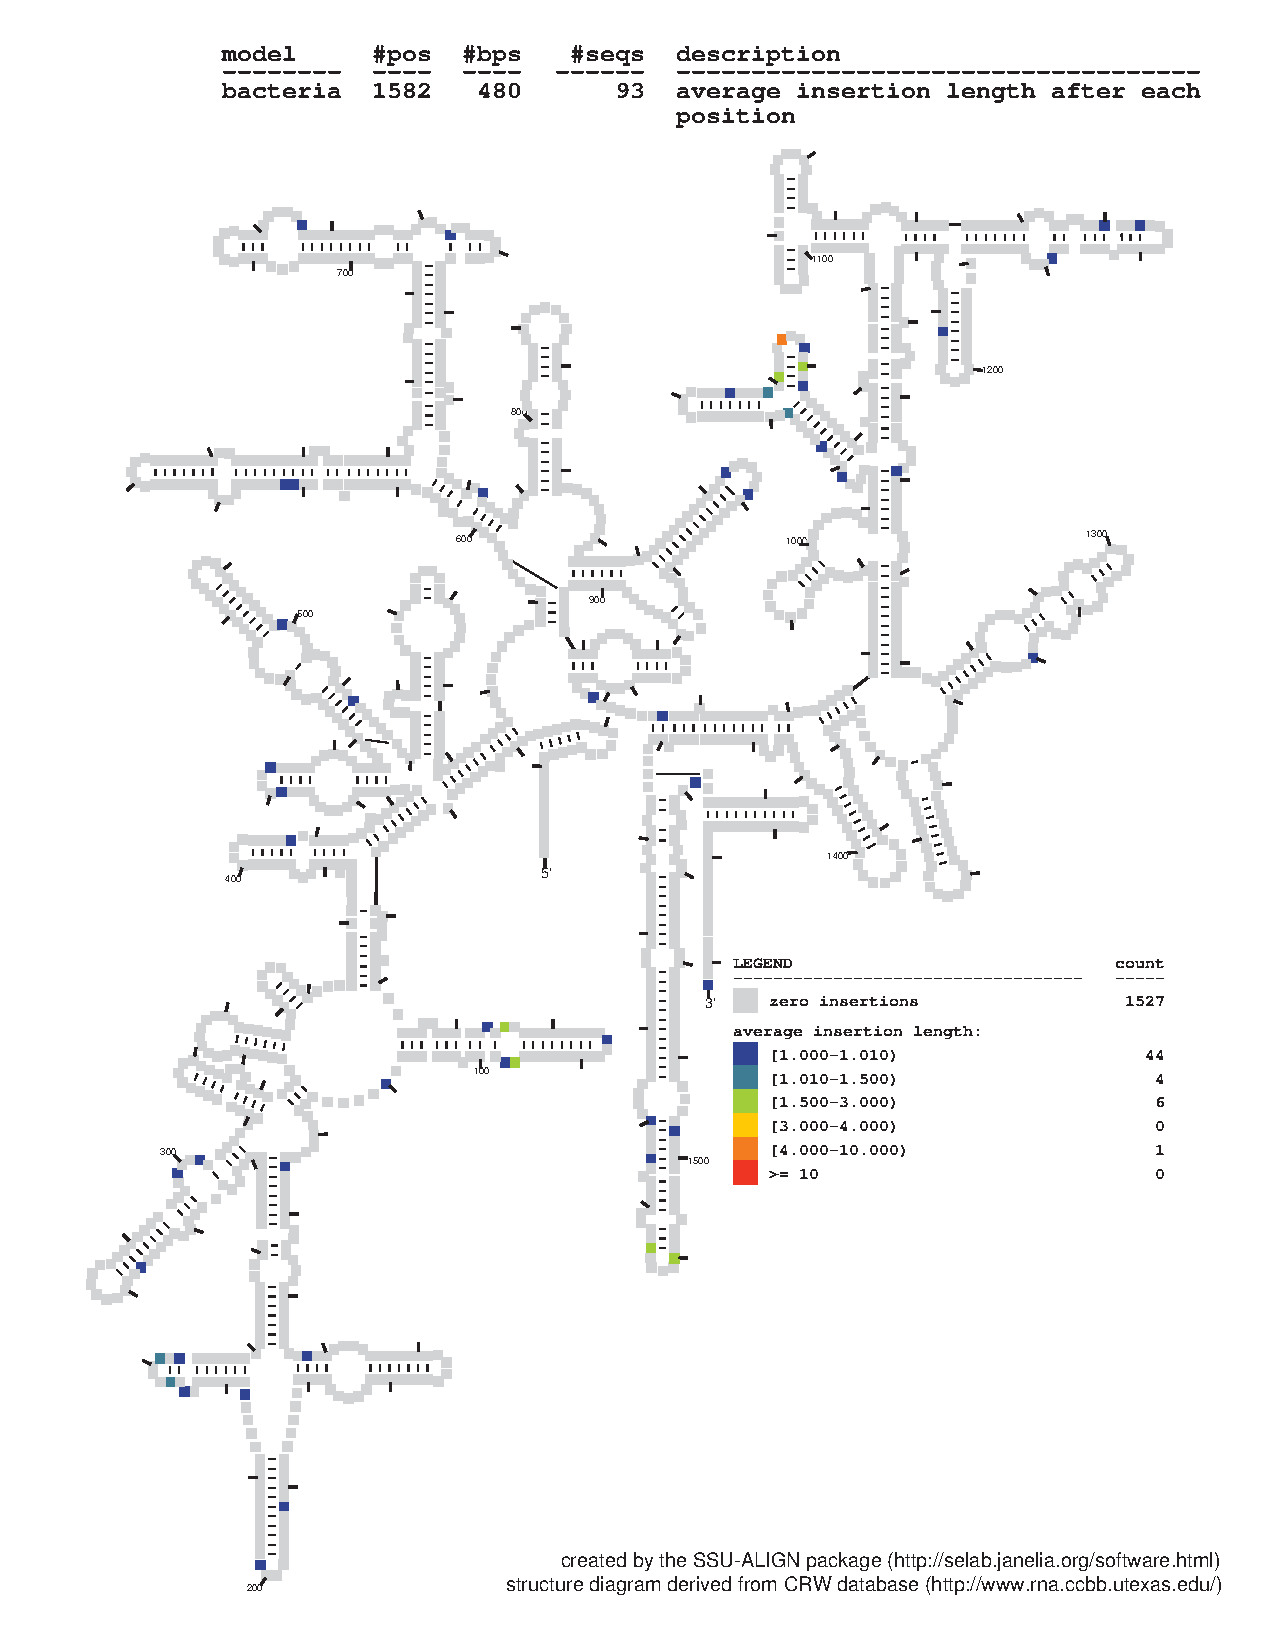
\includegraphics[width=5.64in]{Figures/bacteria-0p1-iavglen}
\end{center}
\caption[Secondary structure diagram displaying average length of insertions
  after each consensus position in the bacterial SSU seed
  alignment]{\textbf{Secondary structure diagram displaying average
    length of insertions after each consensus position in the bacterial SSU seed
  alignment.} Statistics correspond to the SSU-ALIGN seed
  alignment derived from the \db{crw} database \cite{CannoneGutell02}
  as described in the text. This diagram was generated by the {\tt
  ssu-draw} program included in SSU-ALIGN}.
\label{fig:baciavglen}
\end{figure}


%%%%%%%%%%%%%%%%%%%%%%%%%%%%%%%%%%%%%%%%%%%%%%%%%%%%%%%%%%%%%%%%
%eukarya
%%%%%%%%%%%%%%%%%%%%%%%%%%%%%%%%%%%%%%%%%%%%%%%%%%%%%%%%%%%%%%%%
\newpage 
\begin{figure}
\begin{center}
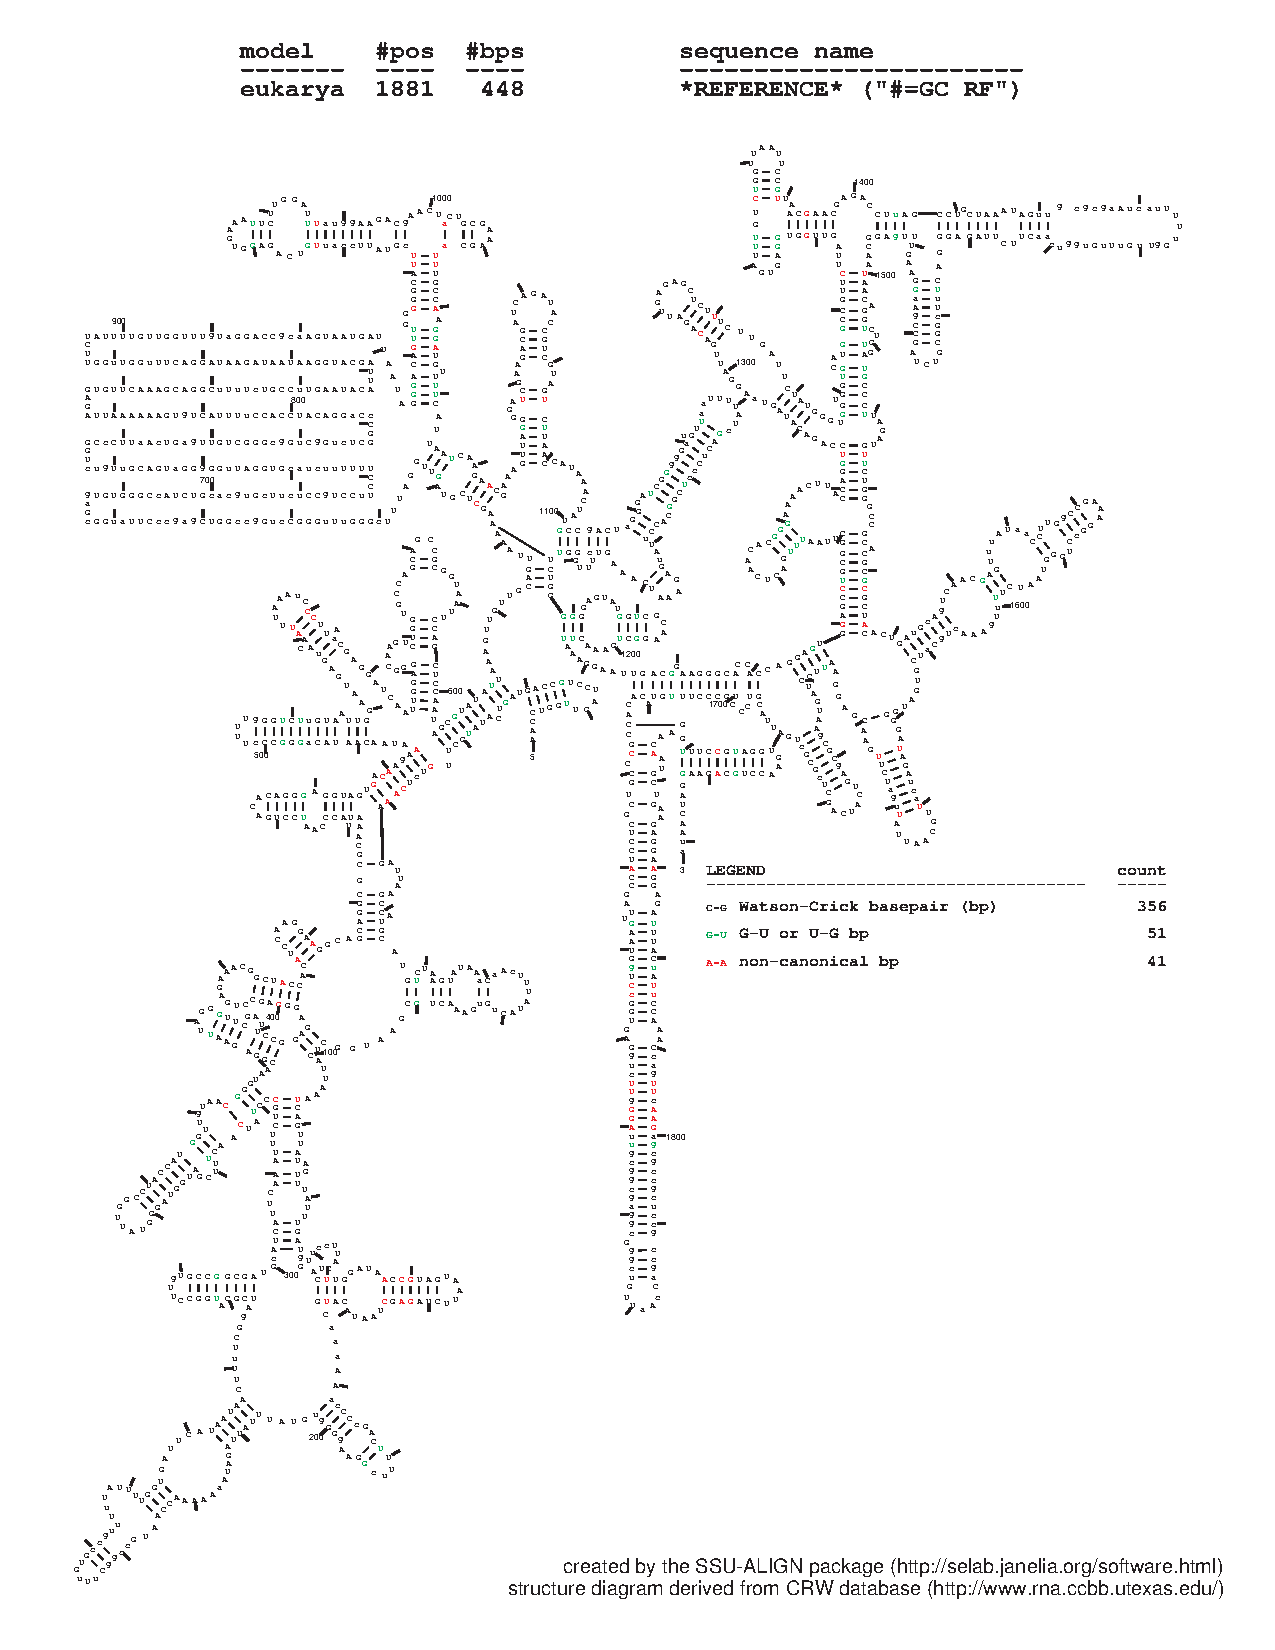
\includegraphics[width=5.64in]{Figures/eukarya-0p1-rf}
\end{center}
\caption[Secondary structure diagram displaying the consensus sequence
  of the eukaryotic SSU model]{\textbf{Secondary structure diagram displaying the
  consensus sequence of the eukaryotic SSU model.} 
  This is the single sequence that the model 
  most closely represents, and is the highest scoring possible
  sequence to the model. Uppercase nucleotides indicate highly conserved positions,
  and lowercase nucleotides indicate less well-conserved positions.
  This diagram was generated by the {\tt
  ssu-draw} program included in SSU-ALIGN}.
\label{fig:eukrf}
\end{figure}

\newpage 

\begin{figure}
\begin{center}
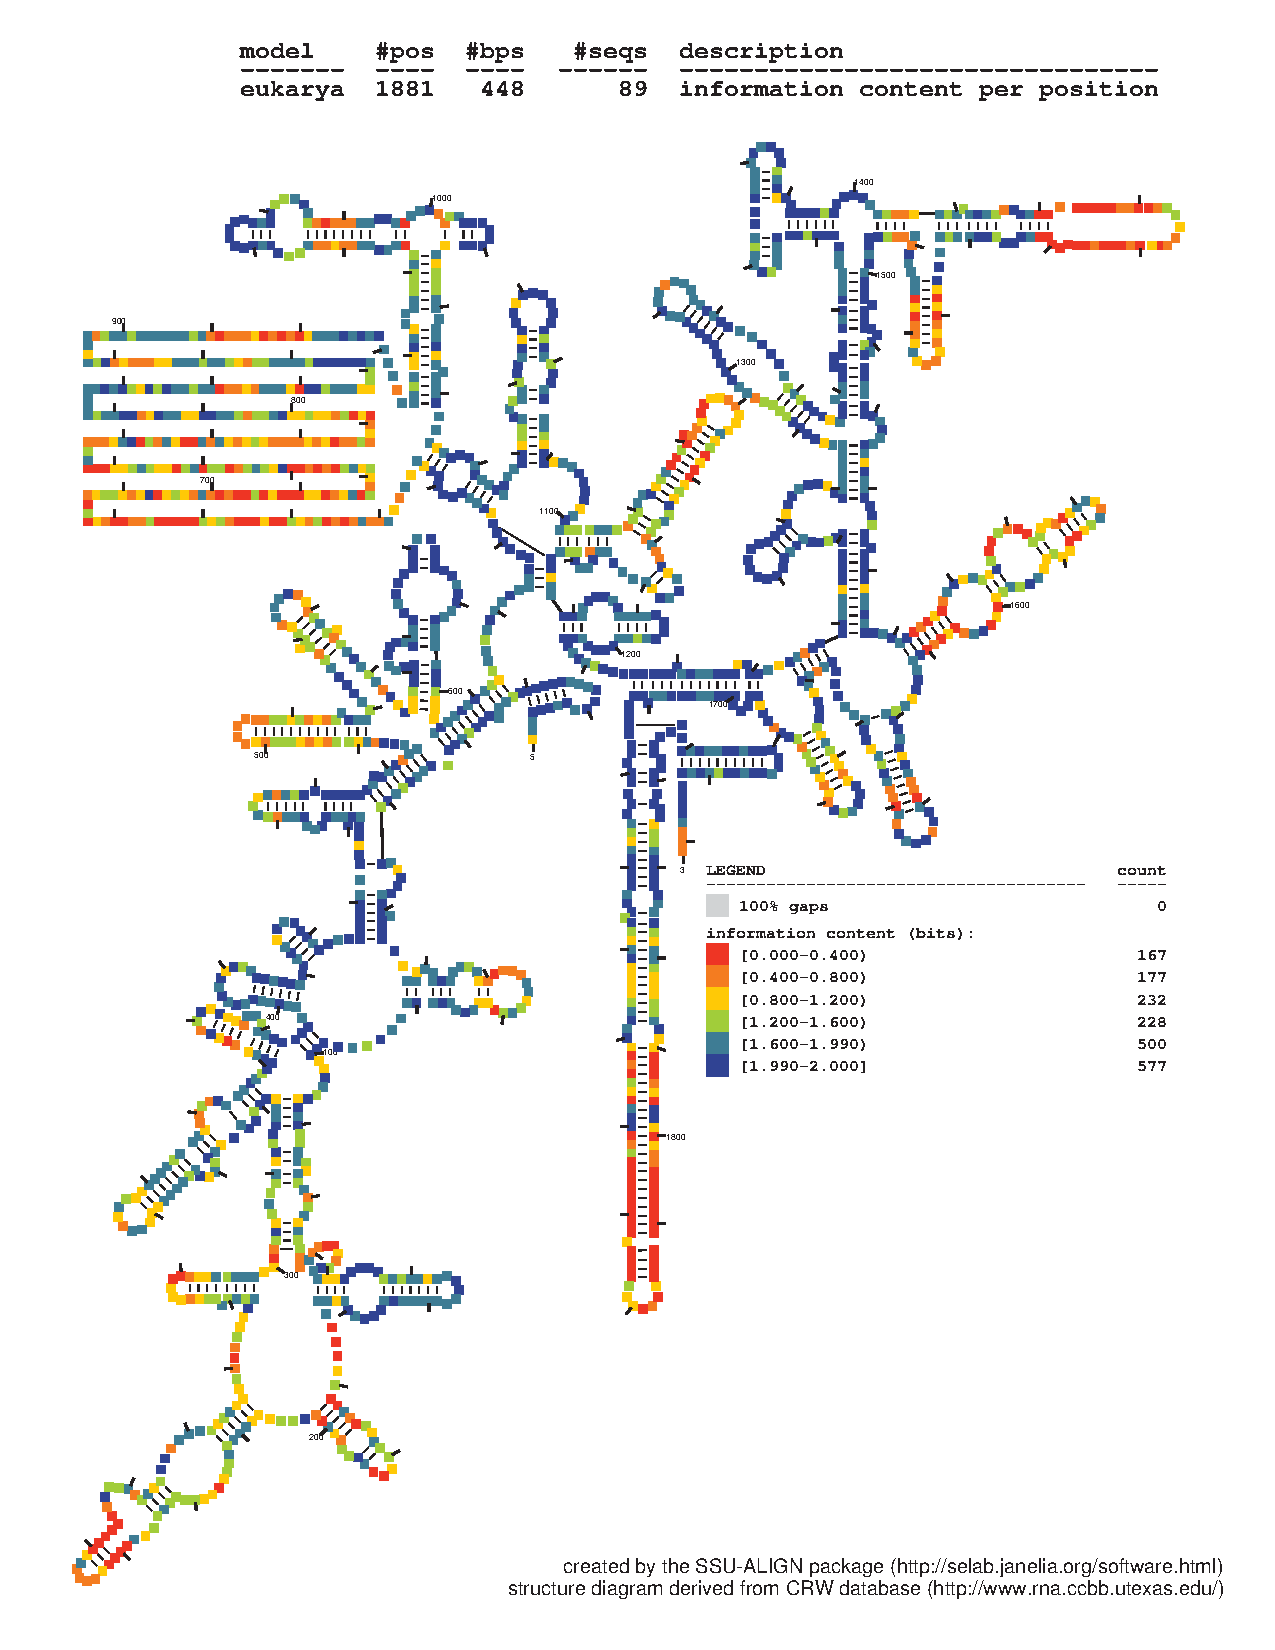
\includegraphics[width=5.64in]{Figures/eukarya-0p1-info}
\end{center}
\caption[Secondary structure diagram displaying primary sequence
  information content per consensus position of the eukaryotic SSU seed
  alignment]{\textbf{Secondary structure diagram displaying primary
  sequence information content per consensus position of the eukaryotic SSU seed
  alignment.} Statistics correspond to the SSU-ALIGN seed
  alignment derived from the \db{crw} database \cite{CannoneGutell02}
  as described in the text. This diagram was generated by the {\tt
  ssu-draw} program included in SSU-ALIGN}.
\label{fig:eukinfo}
\end{figure}

\newpage 

\begin{figure}
\begin{center}
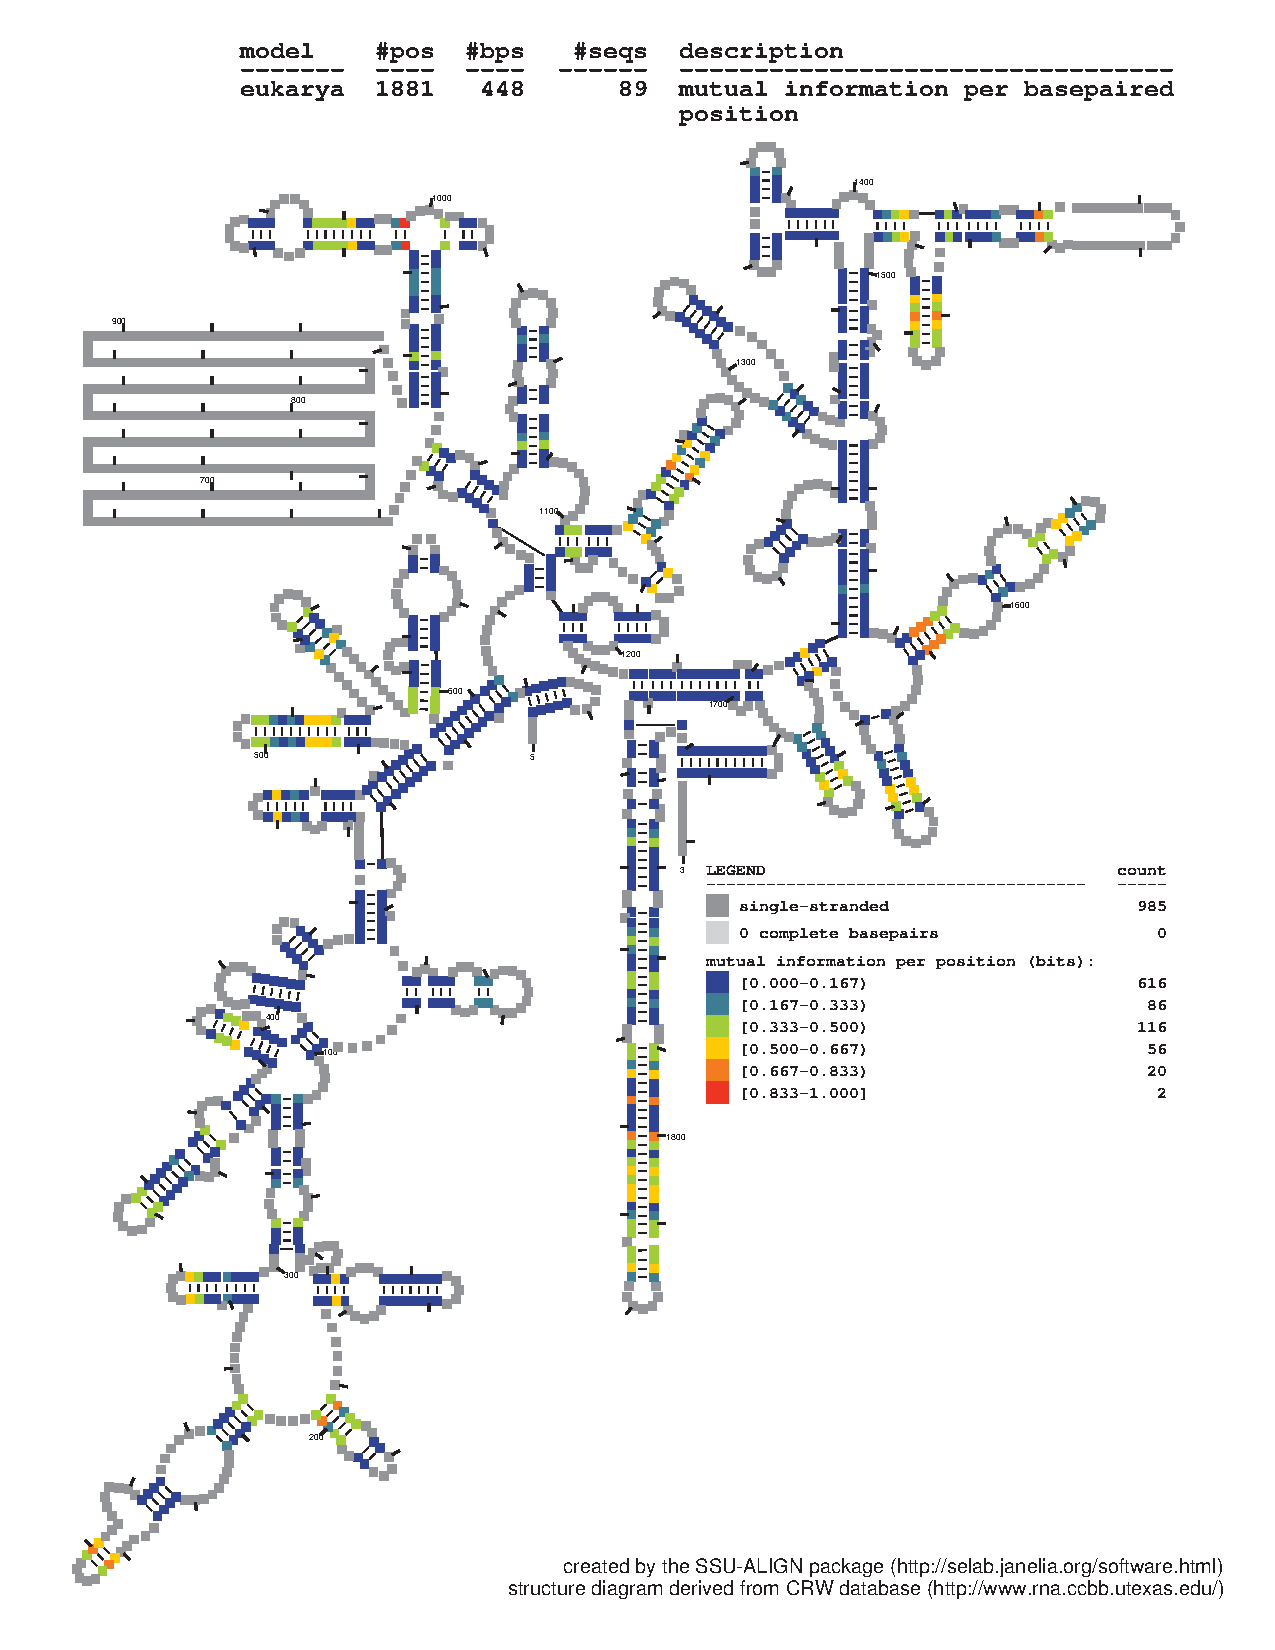
\includegraphics[width=5.64in]{Figures/eukarya-0p1-mutinfo}
\end{center}
\caption[Secondary structure diagram displaying extra information 
  from conserved structure per consensus position of the eukaryotic SSU seed
  alignment]{\textbf{Secondary structure diagram displaying extra
  information from conserved structure per consensus position of the eukaryotic SSU seed
  alignment.} Statistics correspond to the SSU-ALIGN seed
  alignment derived from the \db{crw} database \cite{CannoneGutell02}
  as described in the text. This diagram was generated by the {\tt
  ssu-draw} program included in SSU-ALIGN}.
\label{fig:euksinfo}
\end{figure}

\newpage 

\begin{figure}
\begin{center}
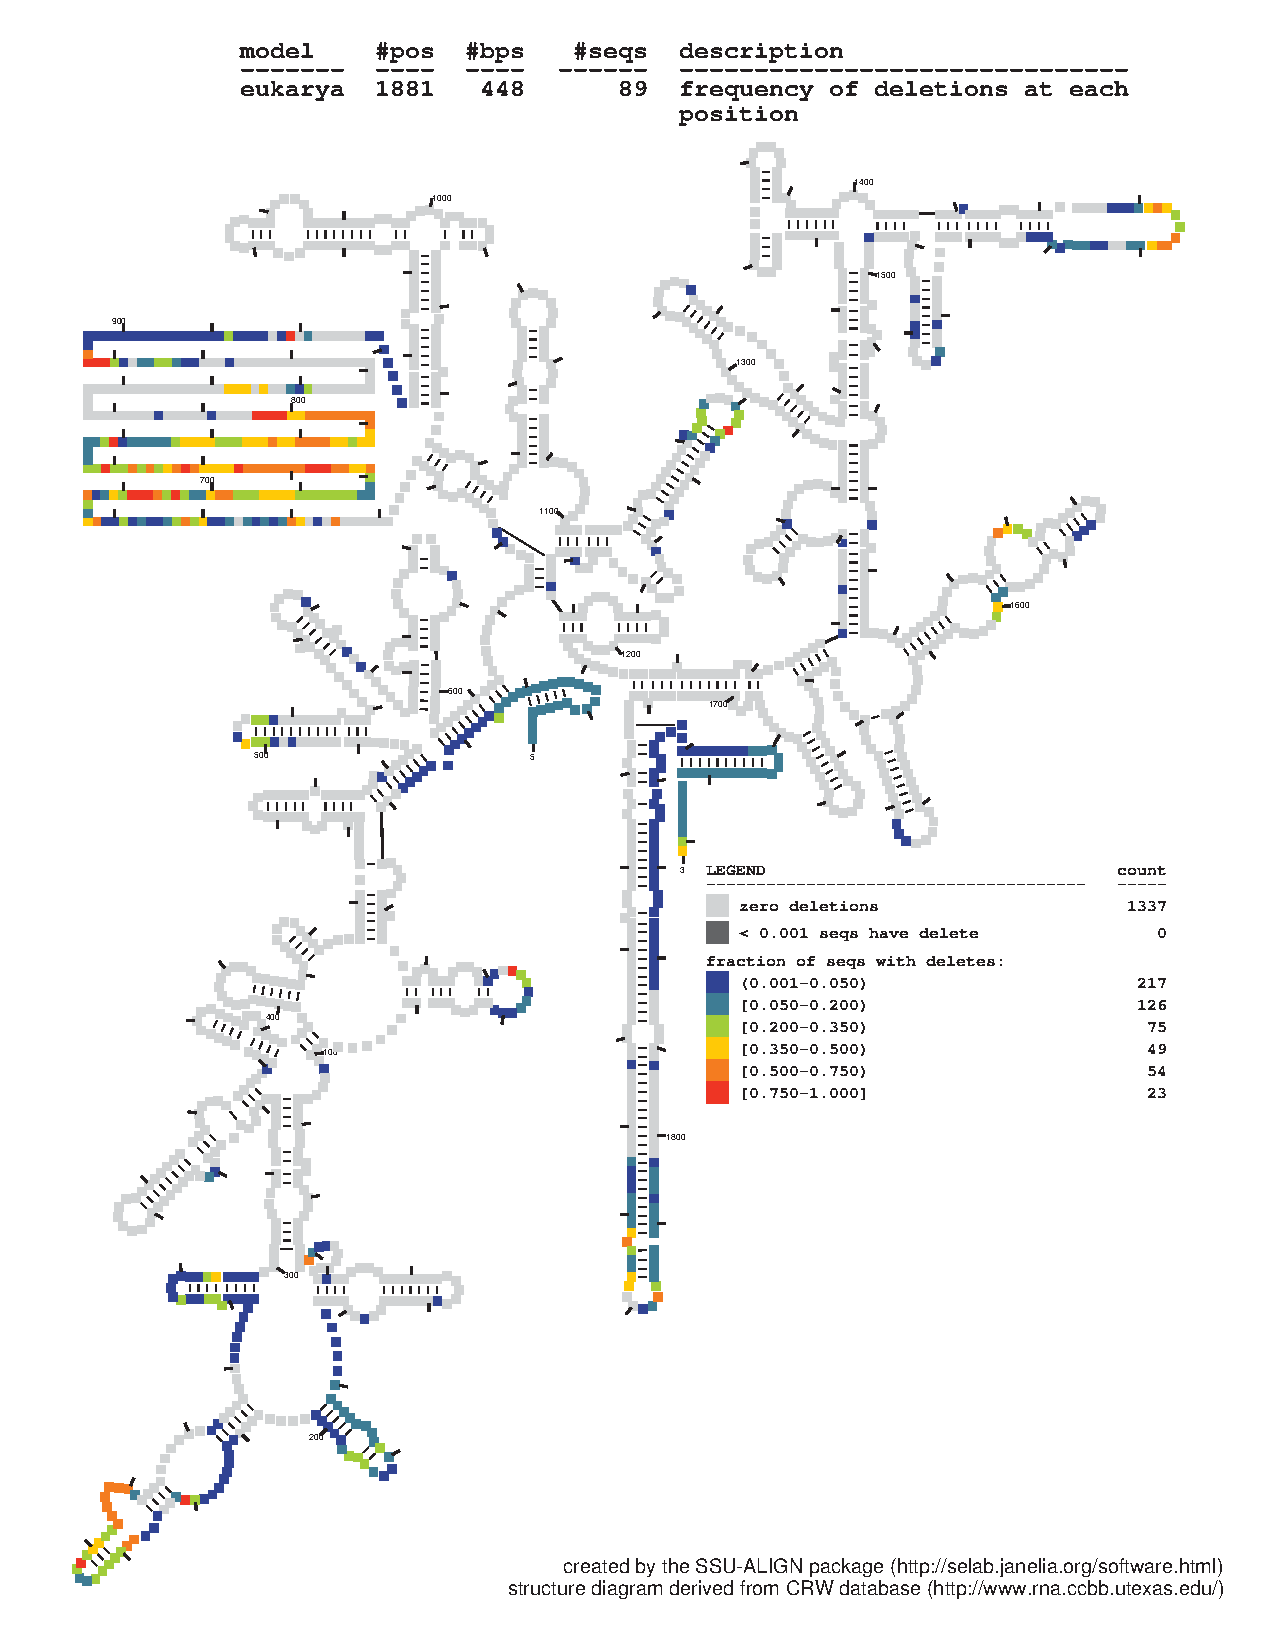
\includegraphics[width=5.64in]{Figures/eukarya-0p1-dall}
\end{center}
\caption[Secondary structure diagram displaying frequency of deletions
  per consensus position of the eukaryotic SSU seed
  alignment]{\textbf{Secondary structure diagram displaying frequency 
  of deletions per consensus position of the eukaryotic SSU seed
  alignment.} Statistics correspond to the SSU-ALIGN seed
  alignment derived from the \db{crw} database \cite{CannoneGutell02}
  as described in the text. This diagram was generated by the {\tt
  ssu-draw} program included in SSU-ALIGN}.
\label{fig:eukdel}
\end{figure}

\newpage 

\begin{figure}
\begin{center}
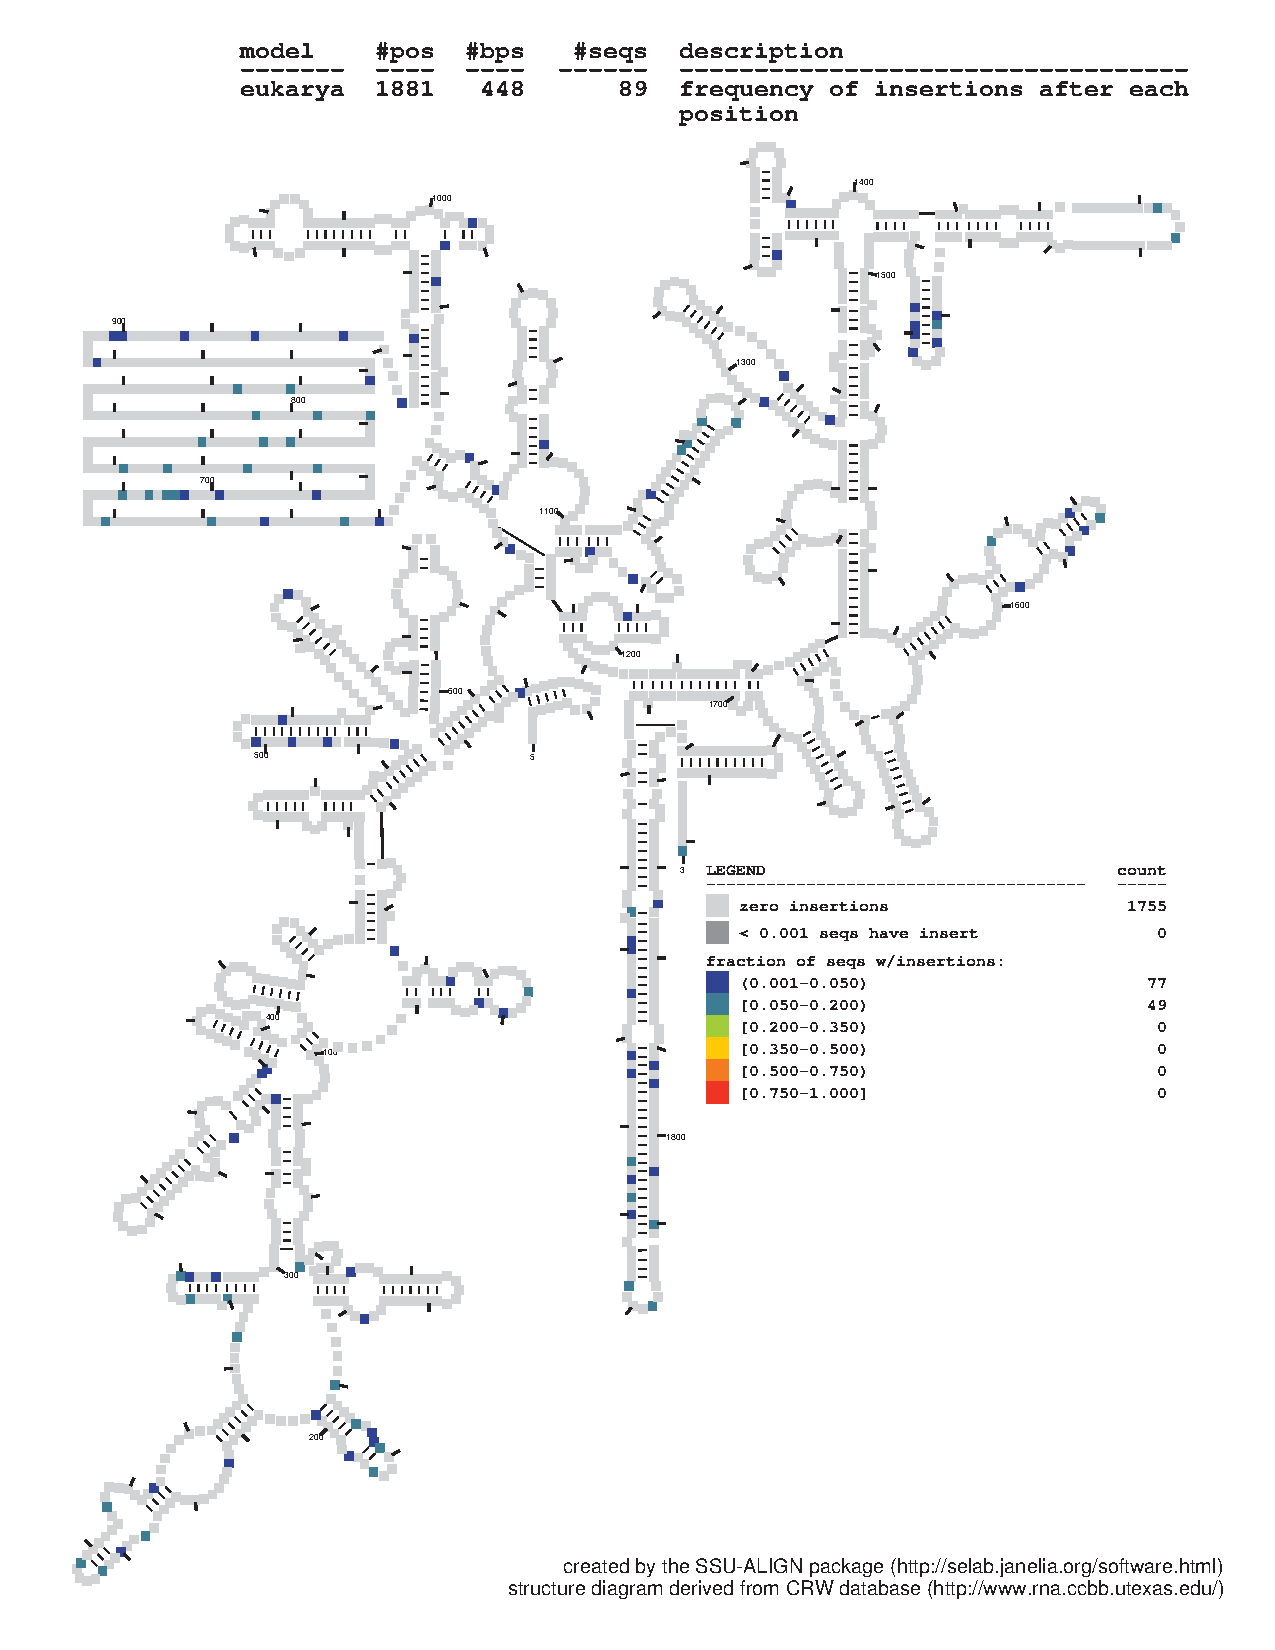
\includegraphics[width=5.64in]{Figures/eukarya-0p1-ifreq}
\end{center}
\caption[Secondary structure diagram displaying frequency of insertions
  after each consensus position in the eukaryotic SSU seed
  alignment]{\textbf{Secondary structure diagram displaying frequency
  of insertions after each consensus position in the eukaryotic SSU seed
  alignment.} Statistics correspond to the SSU-ALIGN seed
  alignment derived from the \db{crw} database \cite{CannoneGutell02}
  as described in the text. This diagram was generated by the {\tt
  ssu-draw} program included in SSU-ALIGN}.
\label{fig:eukifreq}
\end{figure}

\newpage 

\begin{figure}
\begin{center}
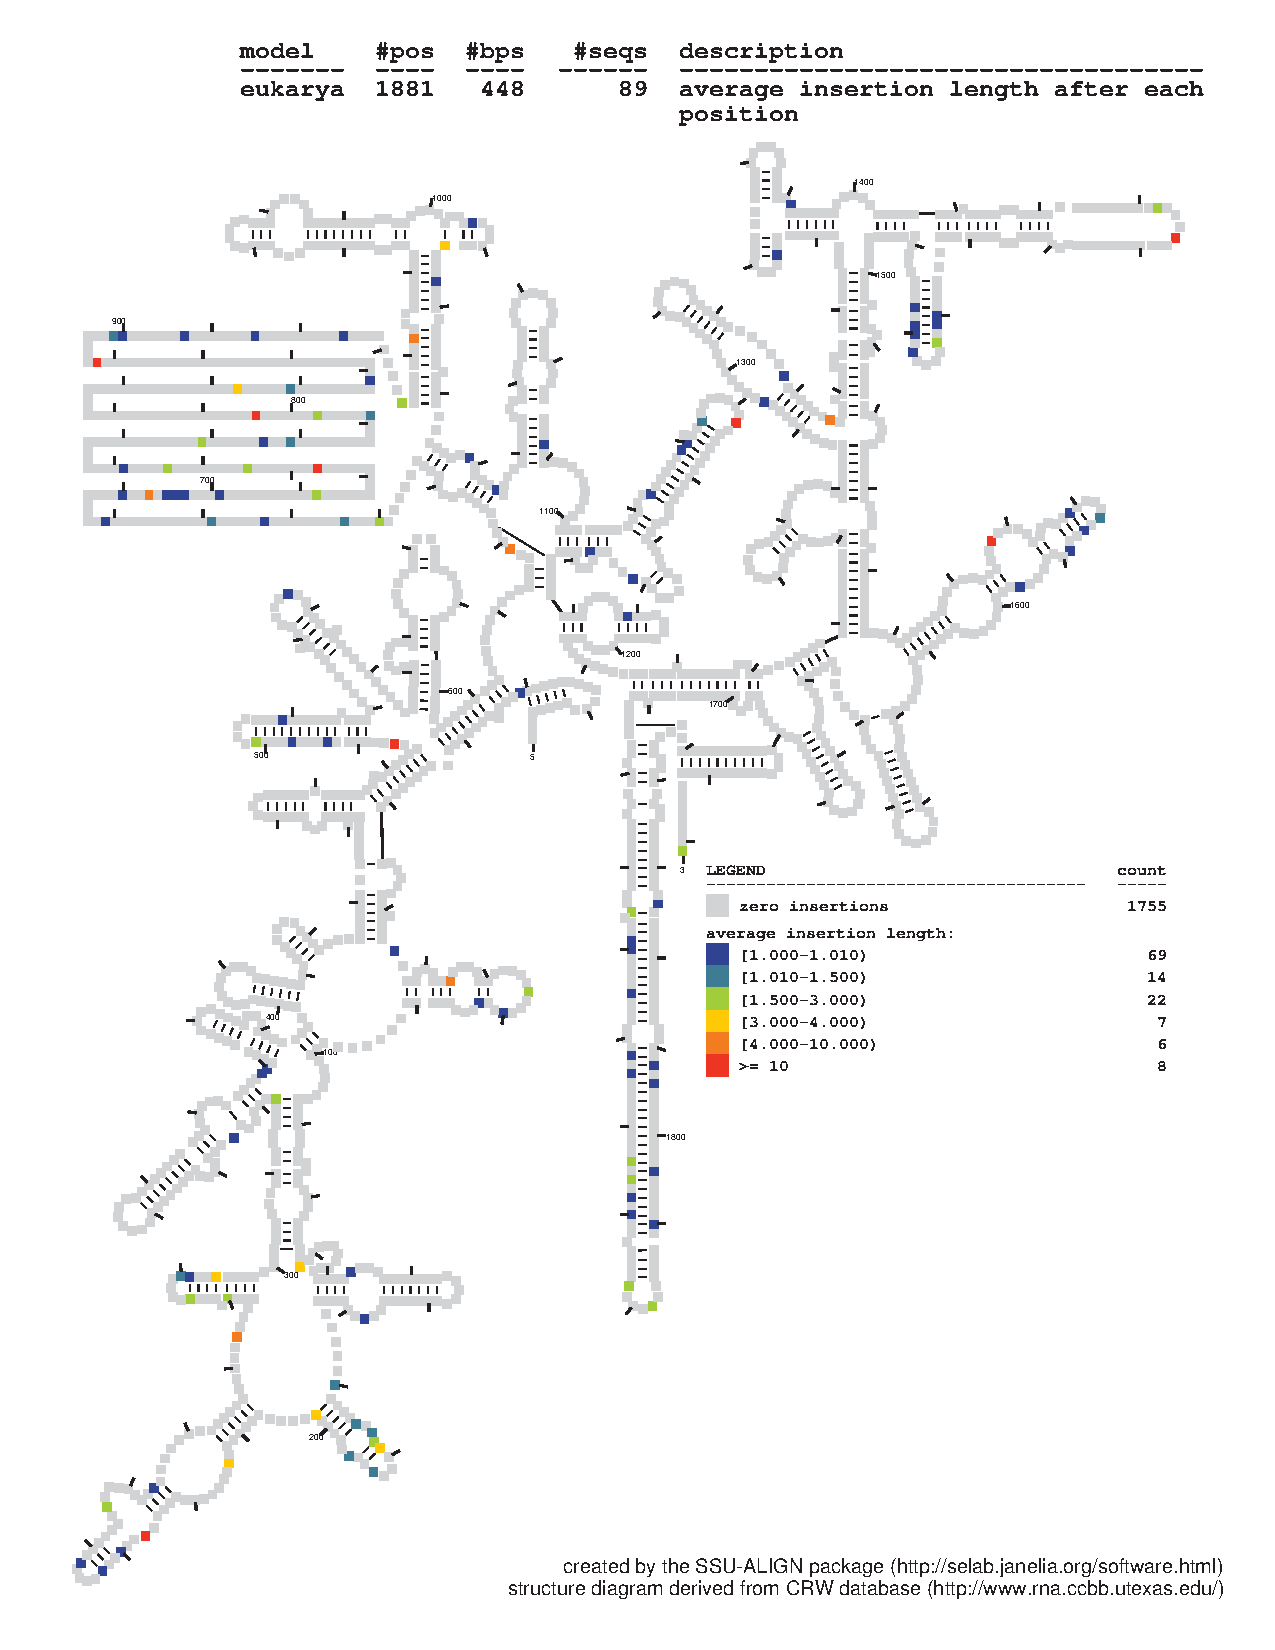
\includegraphics[width=5.64in]{Figures/eukarya-0p1-iavglen}
\end{center}
\caption[Secondary structure diagram displaying average length of insertions
  after each consensus position in the eukaryotic SSU seed
  alignment]{\textbf{Secondary structure diagram displaying average
    length of insertions after each consensus position in the eukaryotic SSU seed
  alignment.} Statistics correspond to the SSU-ALIGN seed
  alignment derived from the \db{crw} database \cite{CannoneGutell02}
  as described in the text. This diagram was generated by the {\tt
  ssu-draw} program included in SSU-ALIGN}.
\label{fig:eukiavglen}
\end{figure}

